\documentclass[doc]{apa6}
%\documentclass{article}
\usepackage{lipsum}
\usepackage[american]{babel}
\usepackage{csquotes}
\usepackage{graphicx}
\usepackage{subfigure}
\usepackage{float}
\usepackage{lineno}



\usepackage[style=apa,sortcites=true,sorting=nyt,backend=biber, uniquename=false, uniquelist=false]{biblatex}
\DeclareLanguageMapping{american}{american-apa}


%\addbibresource{bibliography.bib}



\title{Data Sanity-check Report}


\author{People}

\affiliation{Places}


%\authornote{any notes here}

\shorttitle{CRAAAAZY!!}




%\linenumbers
\begin{document}
\maketitle
\section{Data}

\subsection{Asher 2013}

\begin{figure}[H]
	\centering
	\subfigure{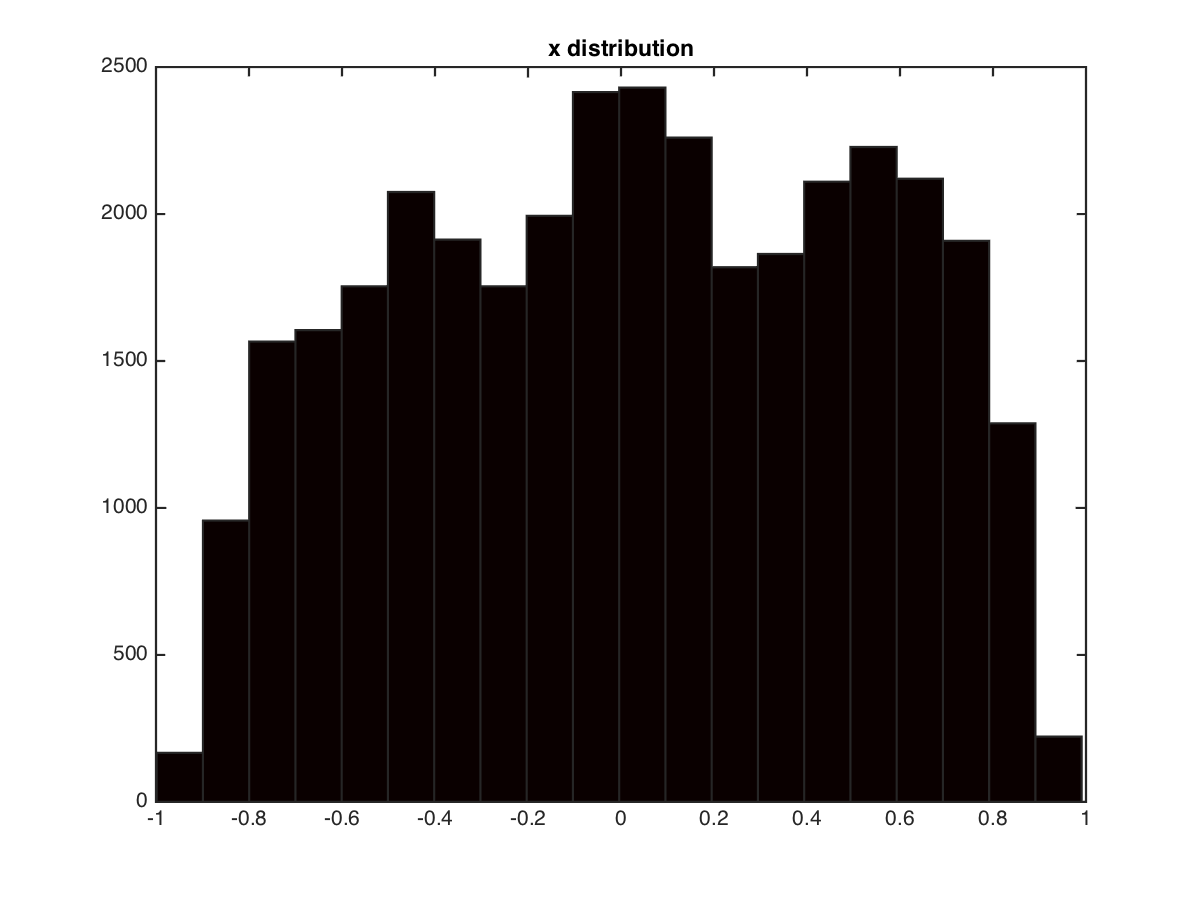
\includegraphics[width=7cm]{Figs/Asher2013_xdist.png}}
	\subfigure{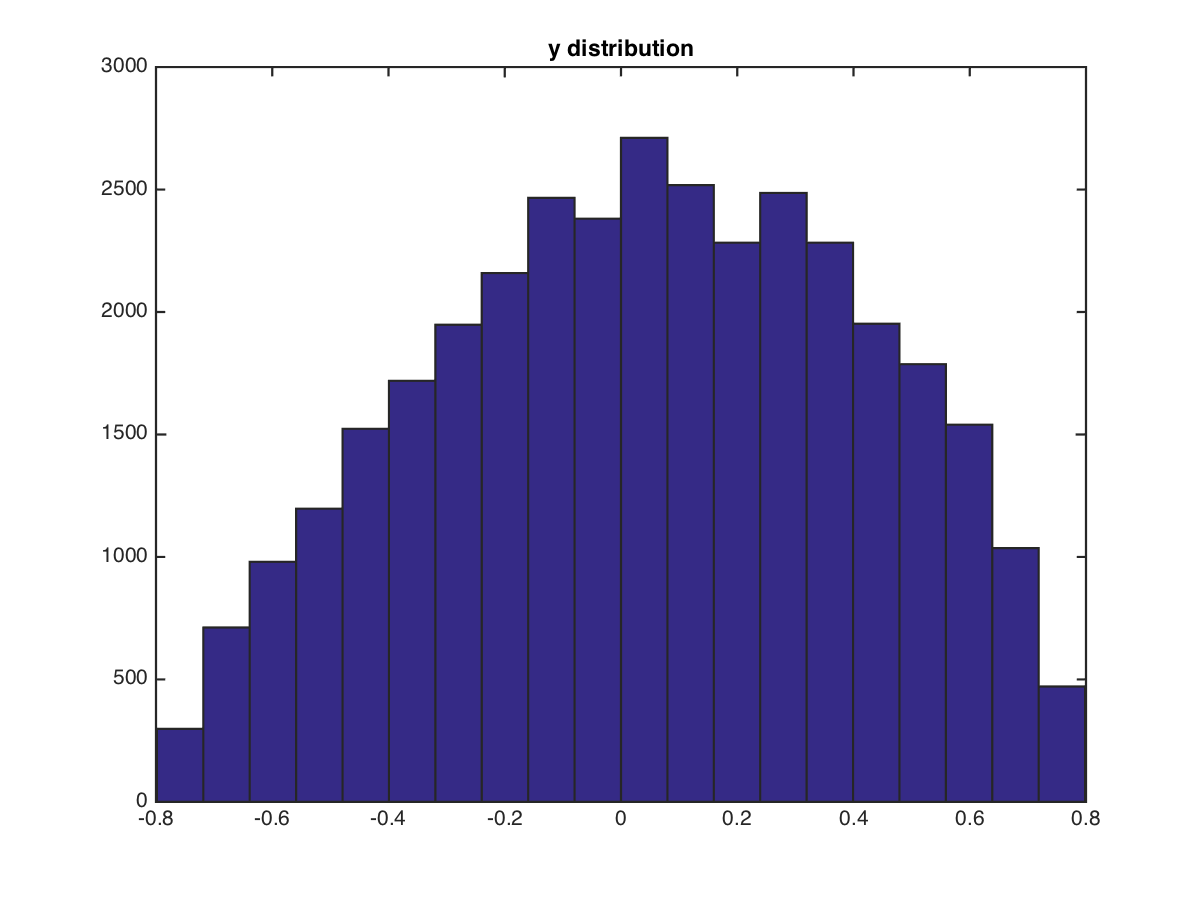
\includegraphics[width=7cm]{Figs/Asher2013_ydist.png}}
	\subfigure{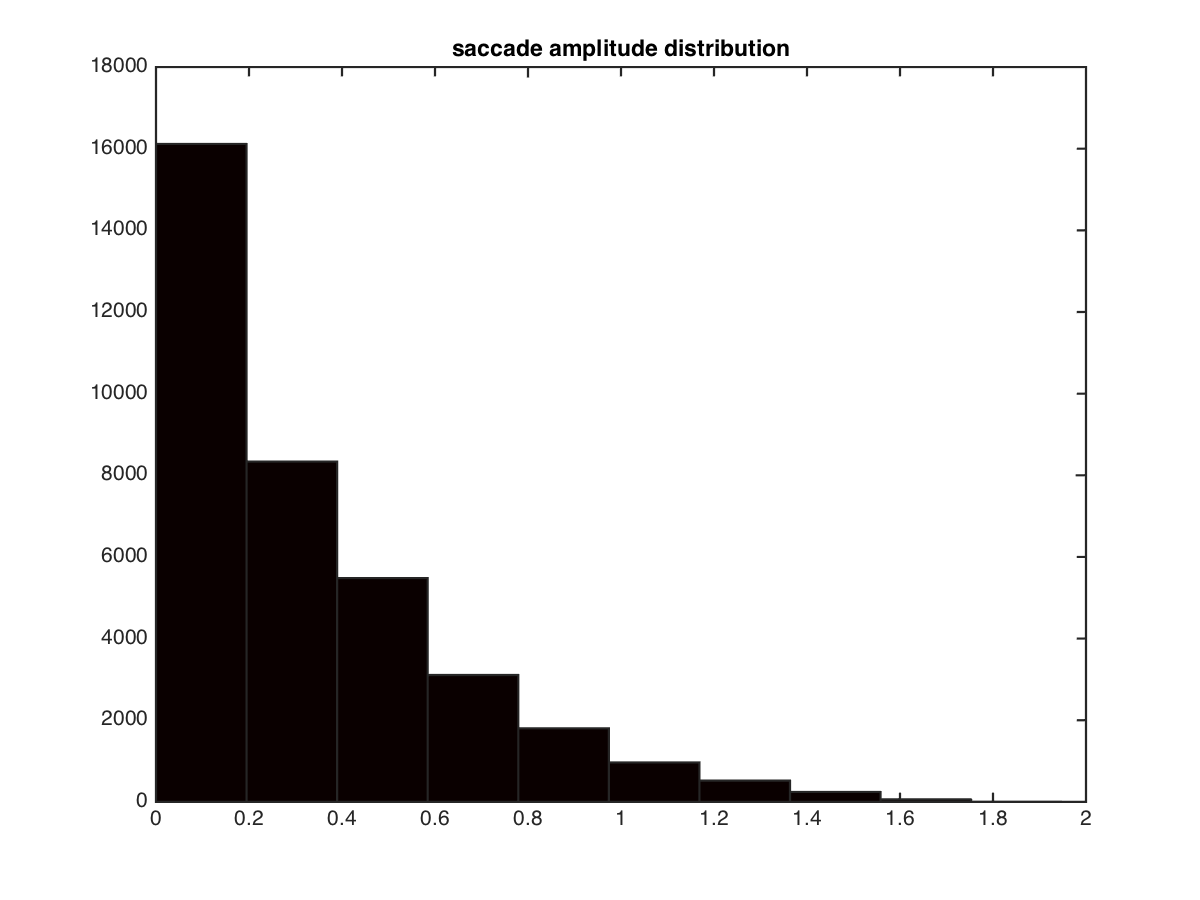
\includegraphics[width=7cm]{Figs/Asher2013_sacampdist.png}}
	\subfigure{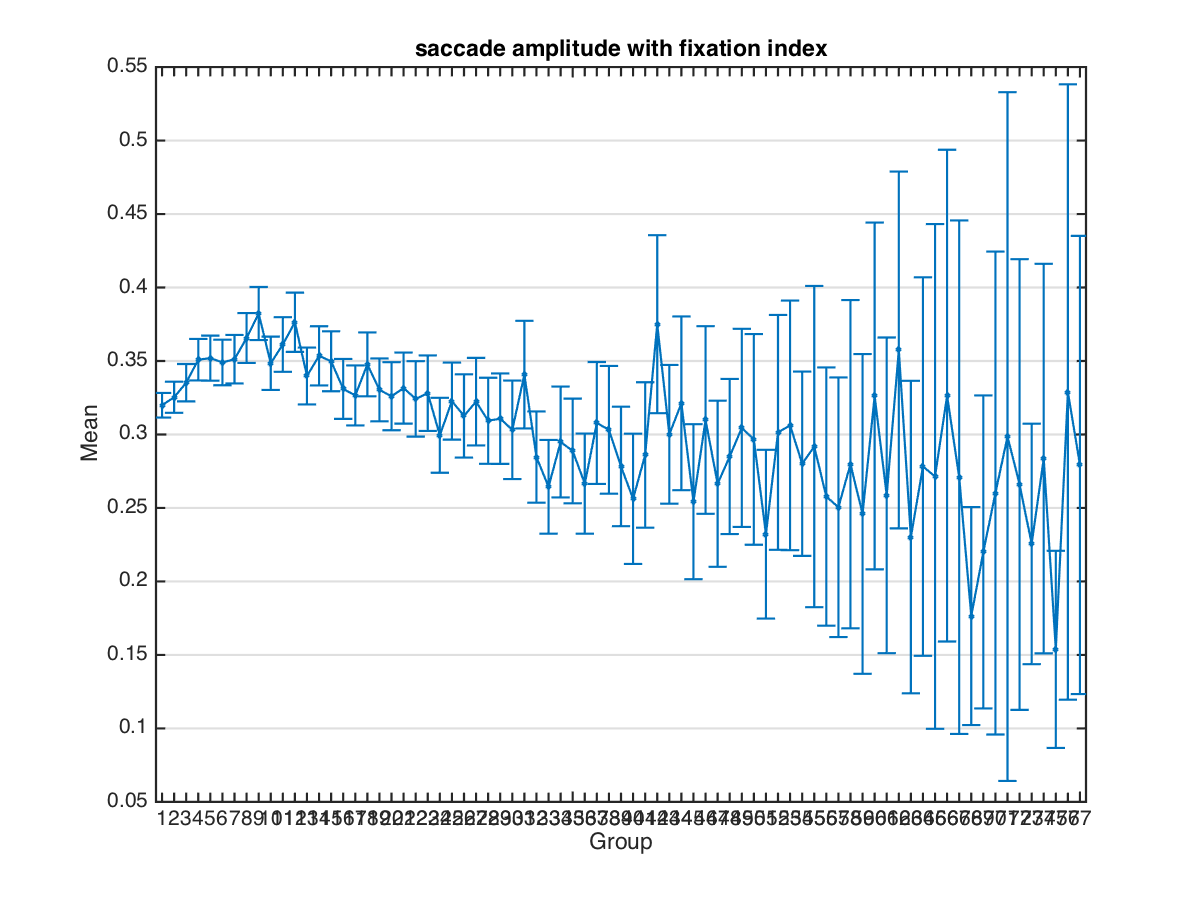
\includegraphics[width=7cm]{Figs/Asher2013_sacampindex.png}}
	\subfigure{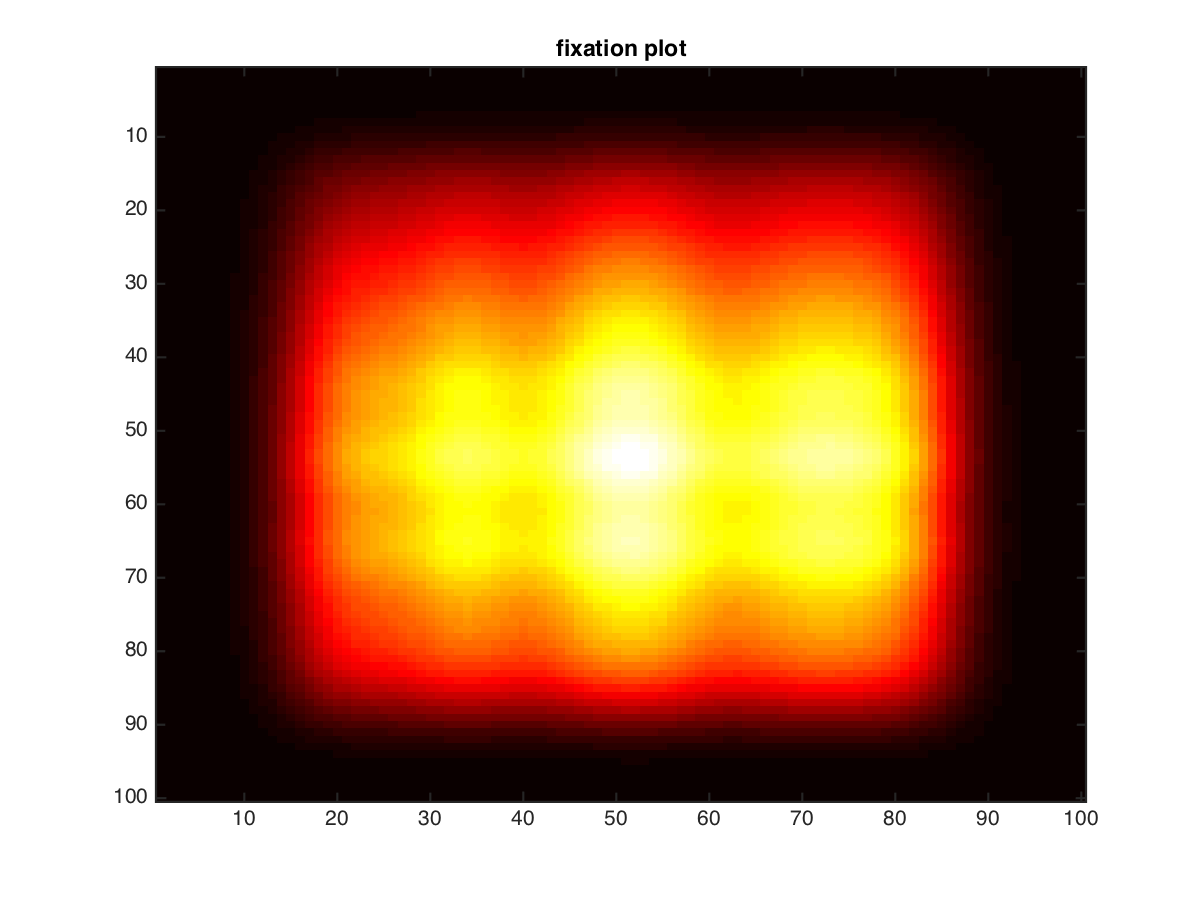
\includegraphics[width=7cm]{Figs/Asher2013_heat.png}}
	\subfigure{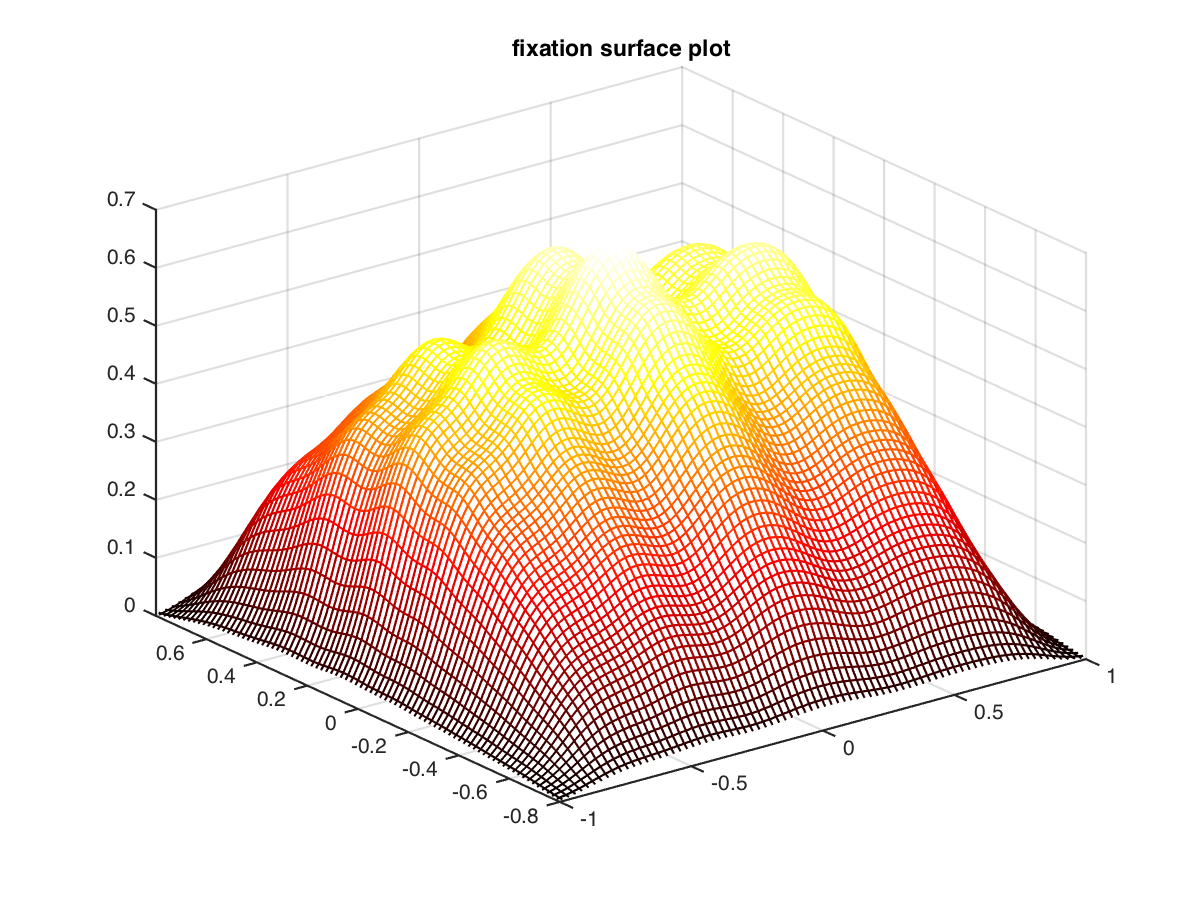
\includegraphics[width=7cm]{Figs/Asher2013_3D.png}}
\caption{Data from Matt Asher 2013}
\label{fig:Asher2013}
\end{figure}

\subsection{Clarke 2013}

\begin{figure}[H]
	\centering
	\subfigure{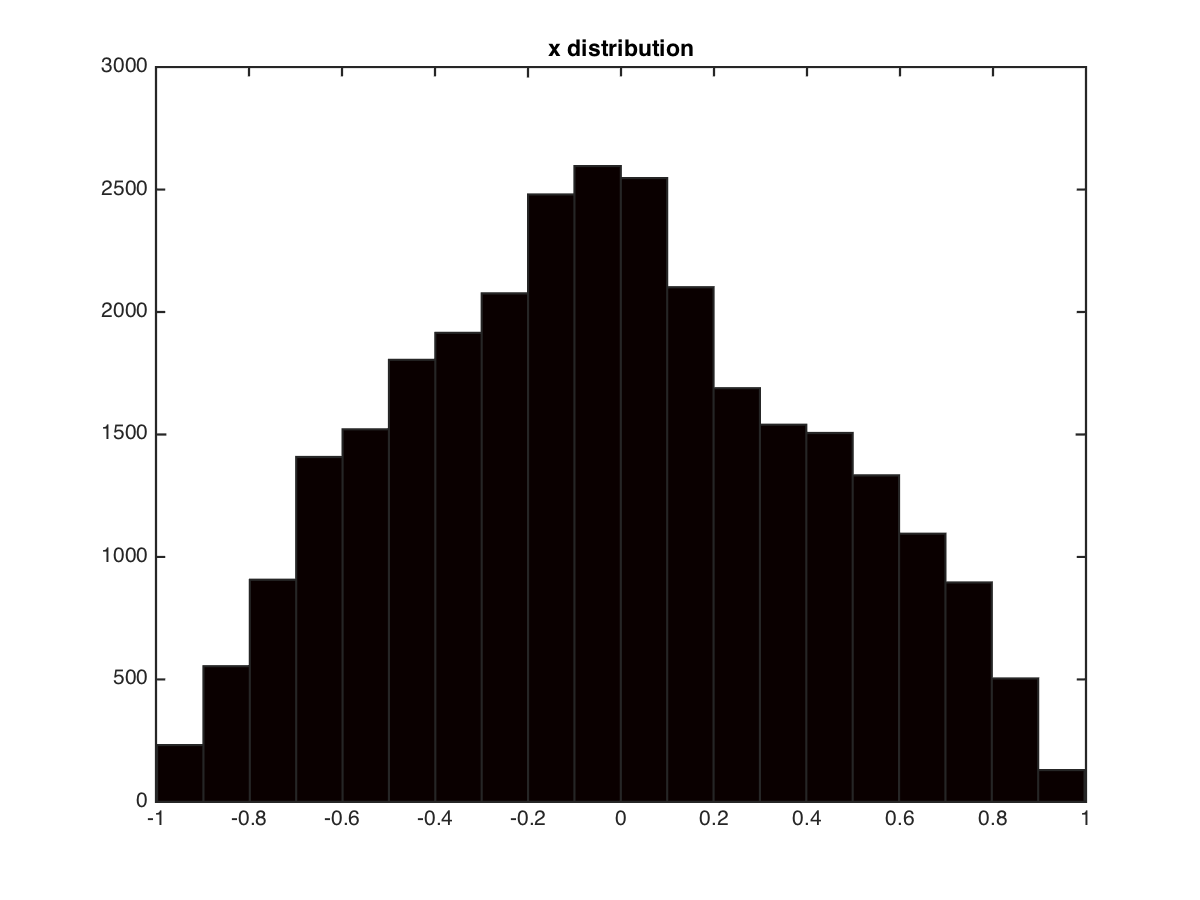
\includegraphics[width=7cm]{Figs/Clarke2013_xdist.png}}
	\subfigure{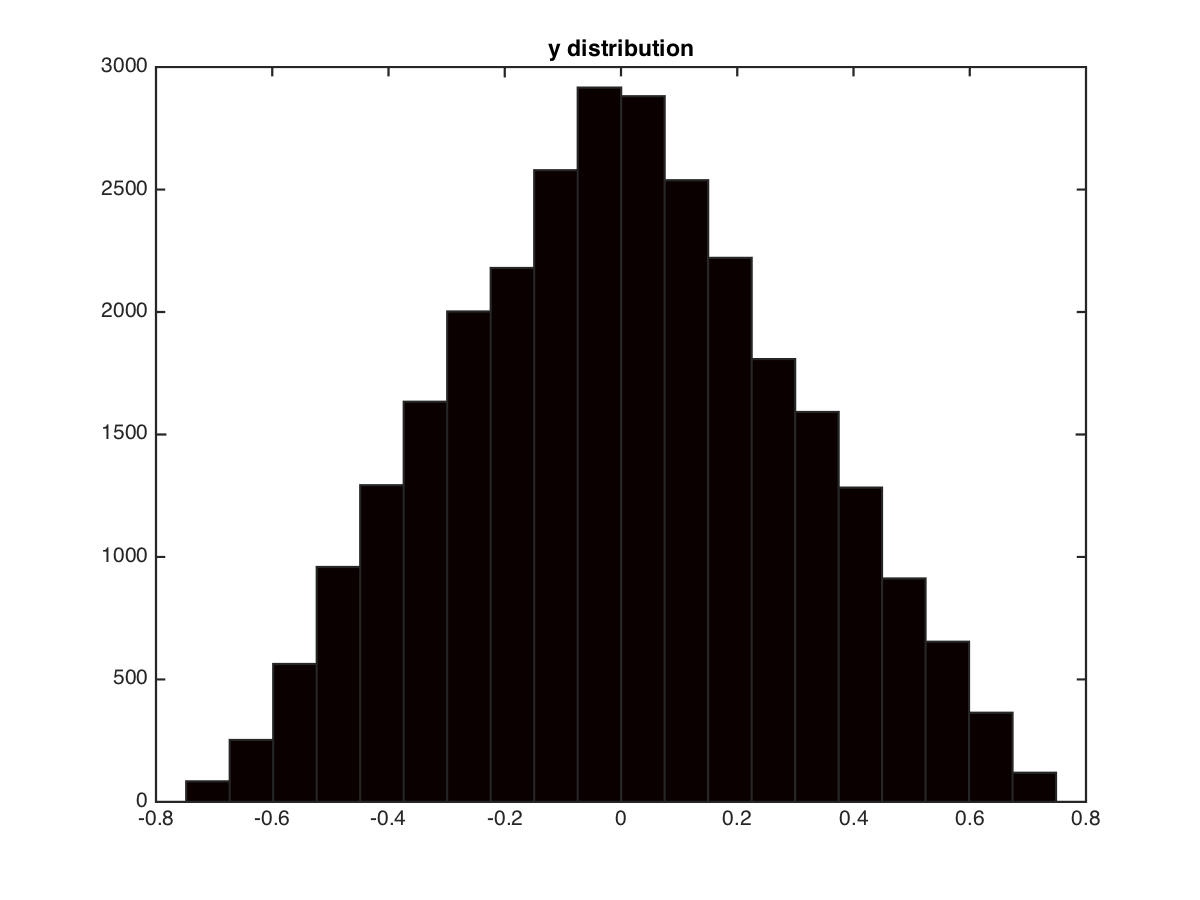
\includegraphics[width=7cm]{Figs/Clarke2013_ydist.png}}
	\subfigure{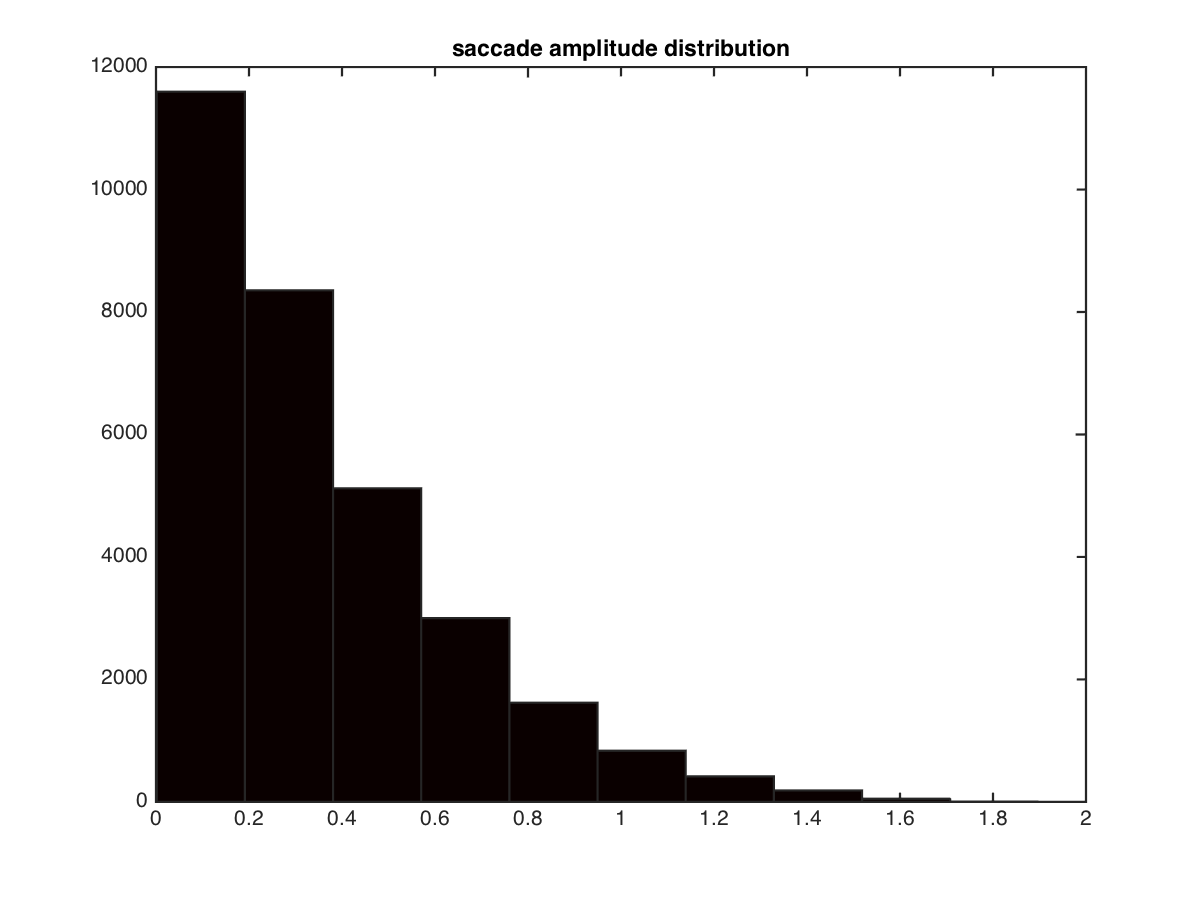
\includegraphics[width=7cm]{Figs/Clarke2013_sacampdist.png}}
	\subfigure{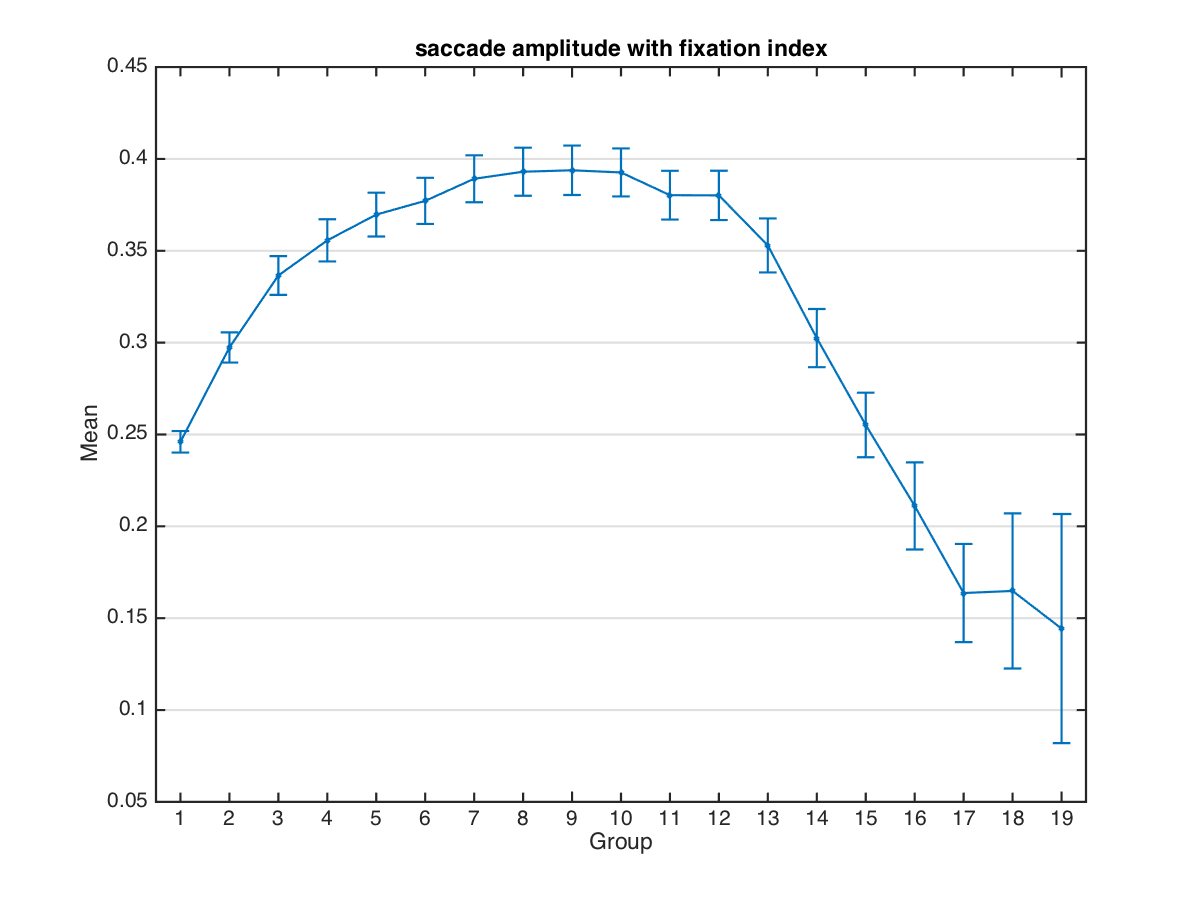
\includegraphics[width=7cm]{Figs/Clarke2013_sacampindex.png}}
	\subfigure{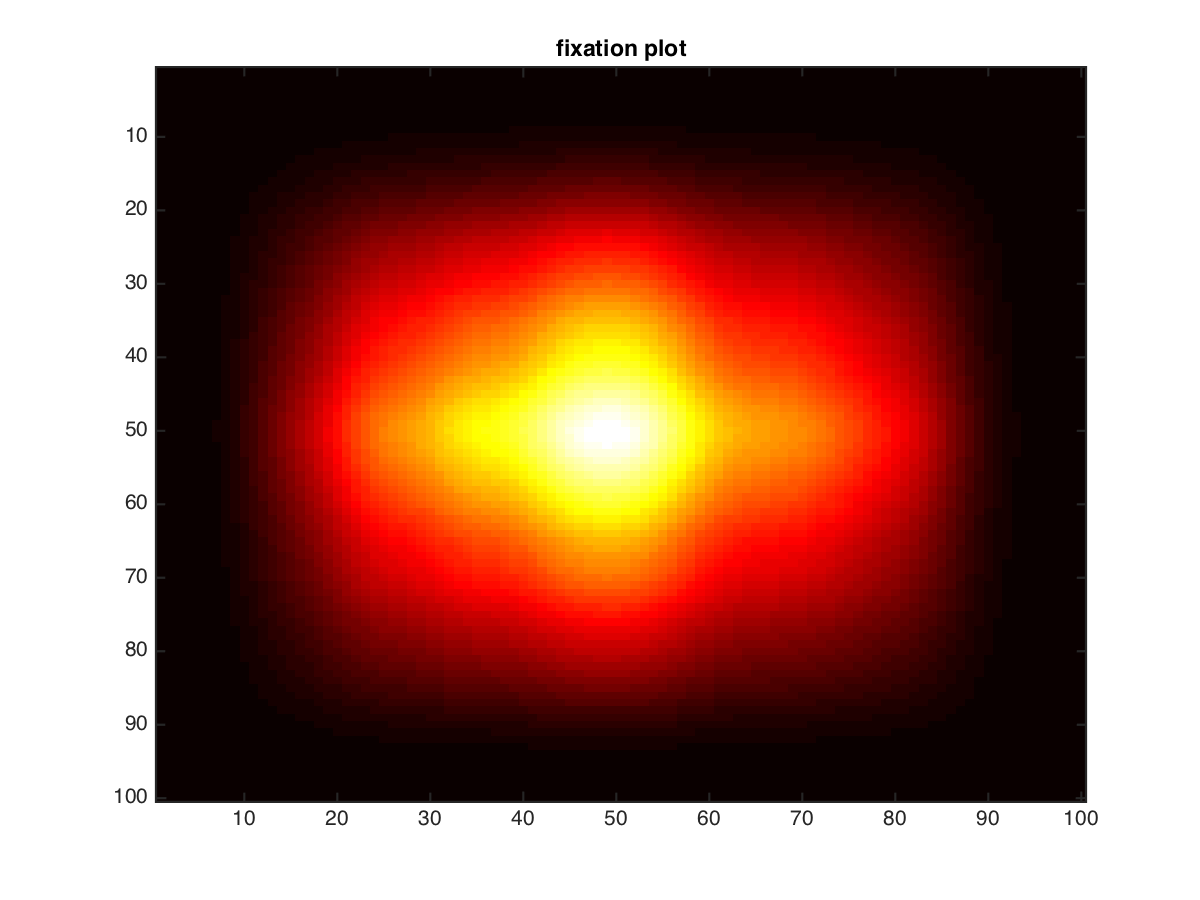
\includegraphics[width=7cm]{Figs/Clarke2013_heat.png}}
	\subfigure{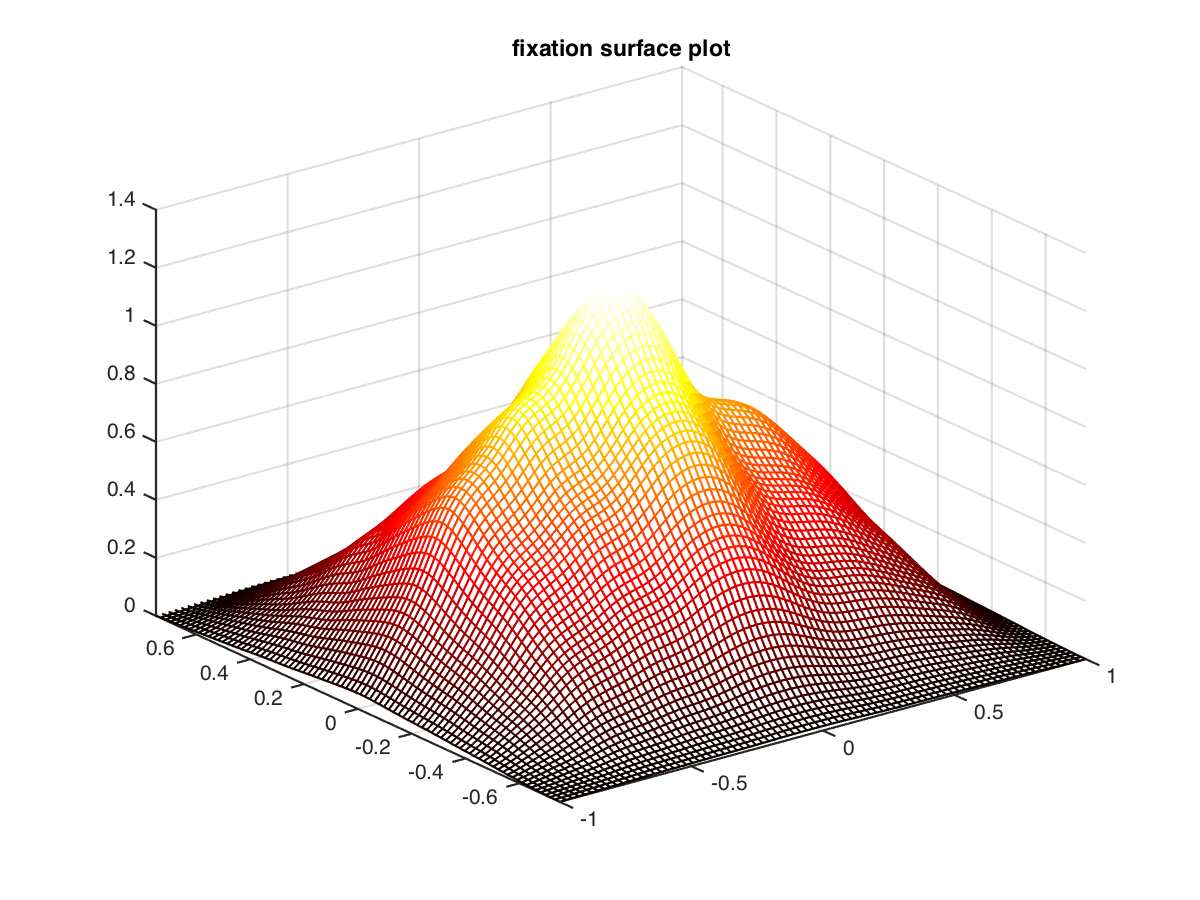
\includegraphics[width=7cm]{Figs/Clarke2013_3D.png}}
\caption{Some guy called Clark's data}
\label{fig:Clarke2013}
\end{figure}


\subsection{Clarke 2009}

\begin{figure}[H]
	\centering
	\subfigure{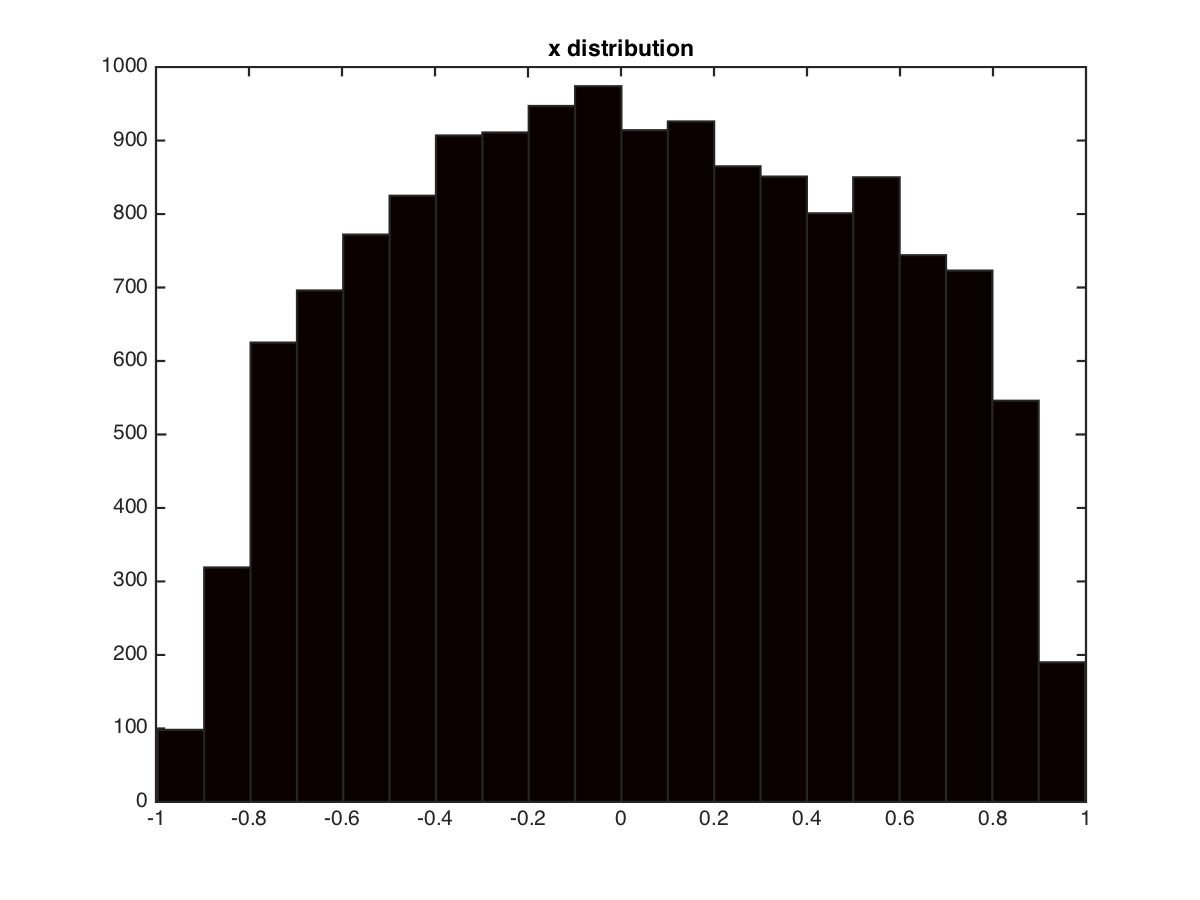
\includegraphics[width=7cm]{Figs/Clarke2009_xdist.png}}
	\subfigure{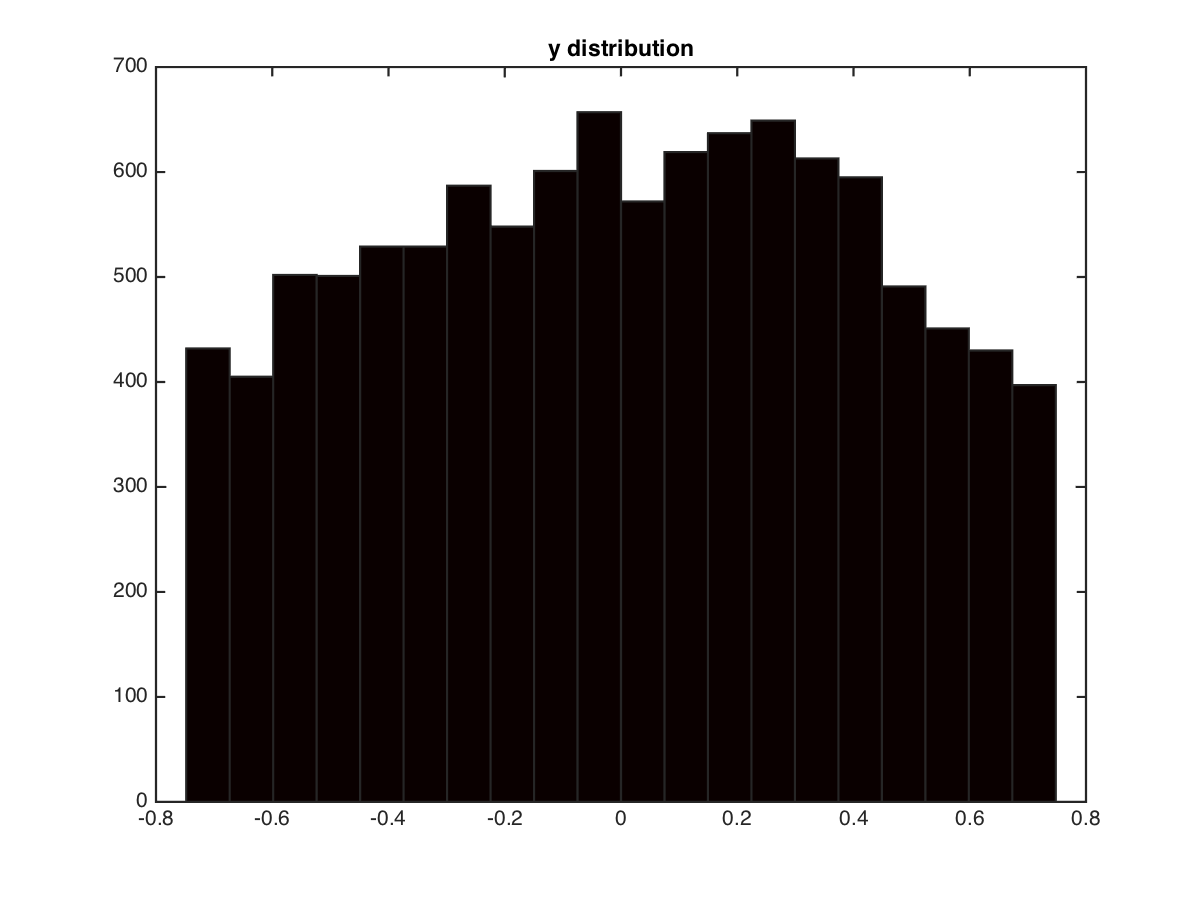
\includegraphics[width=7cm]{Figs/Clarke2009_ydist.png}}
	\subfigure{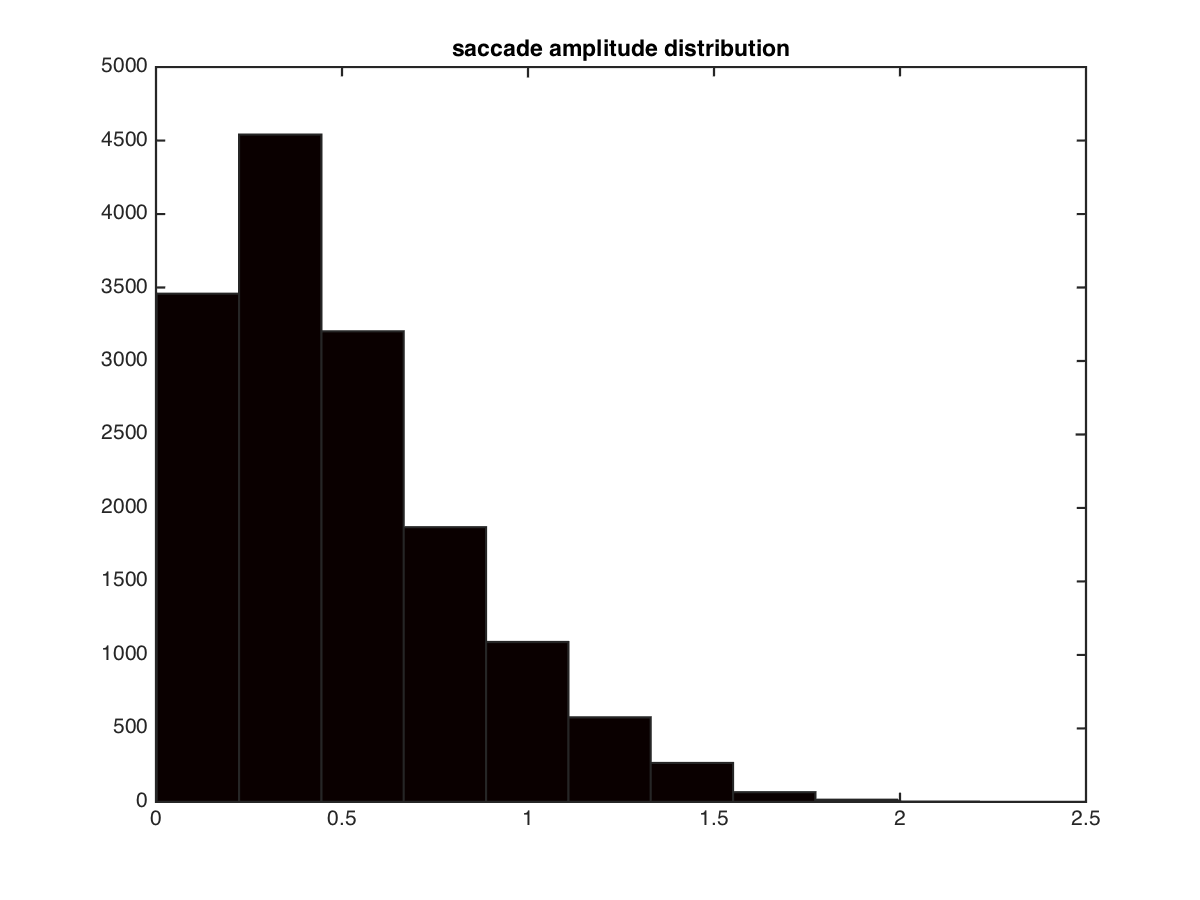
\includegraphics[width=7cm]{Figs/Clarke2009_sacampdist.png}}
	\subfigure{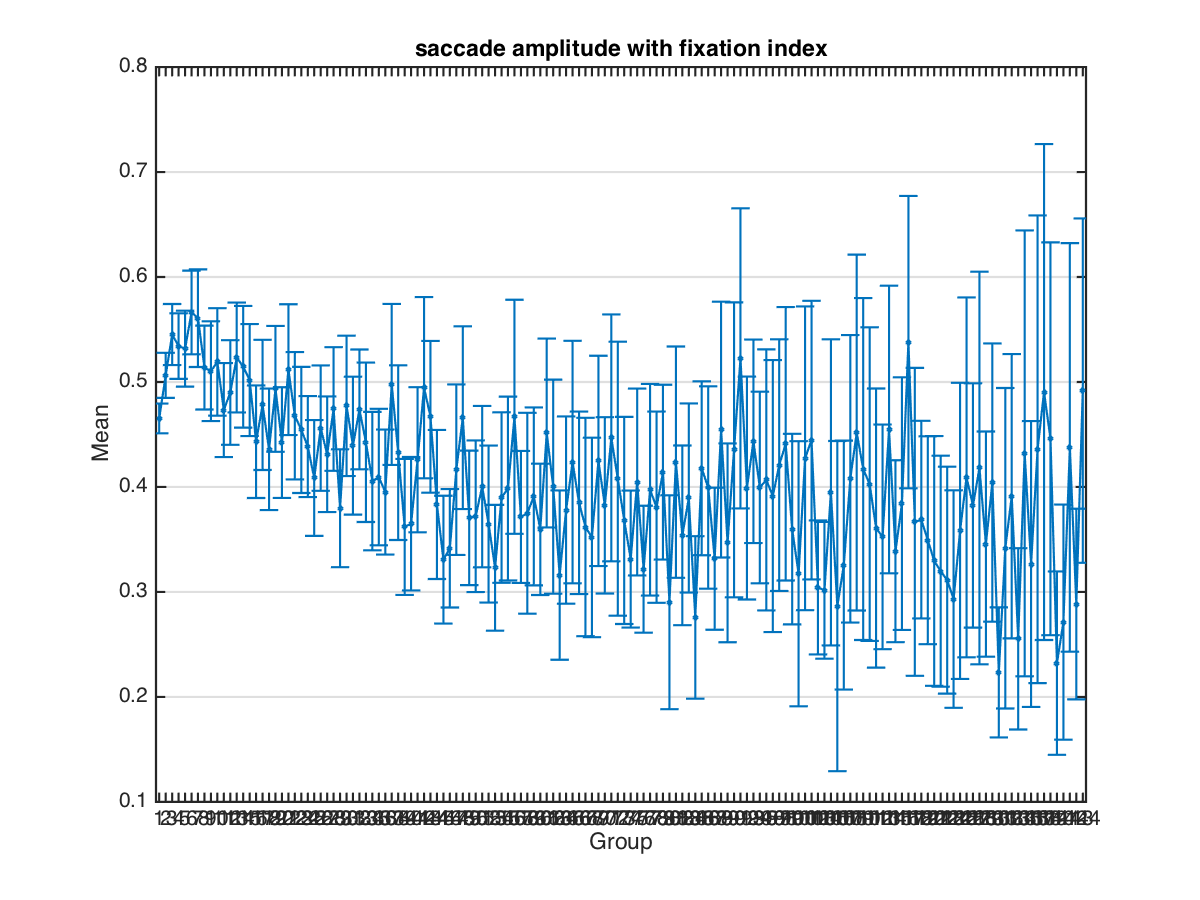
\includegraphics[width=7cm]{Figs/Clarke2009_sacampindex.png}}
	\subfigure{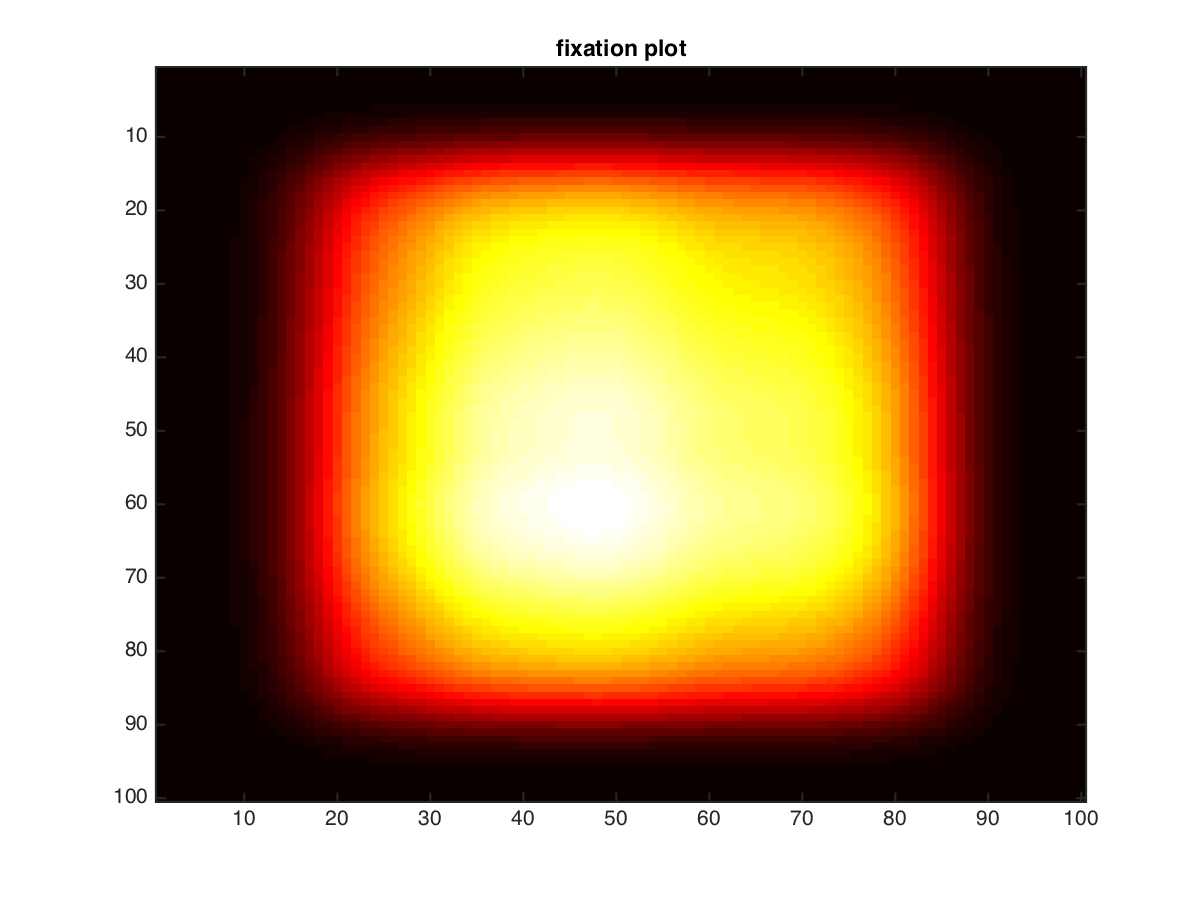
\includegraphics[width=7cm]{Figs/Clarke2009_heat.png}}
	\subfigure{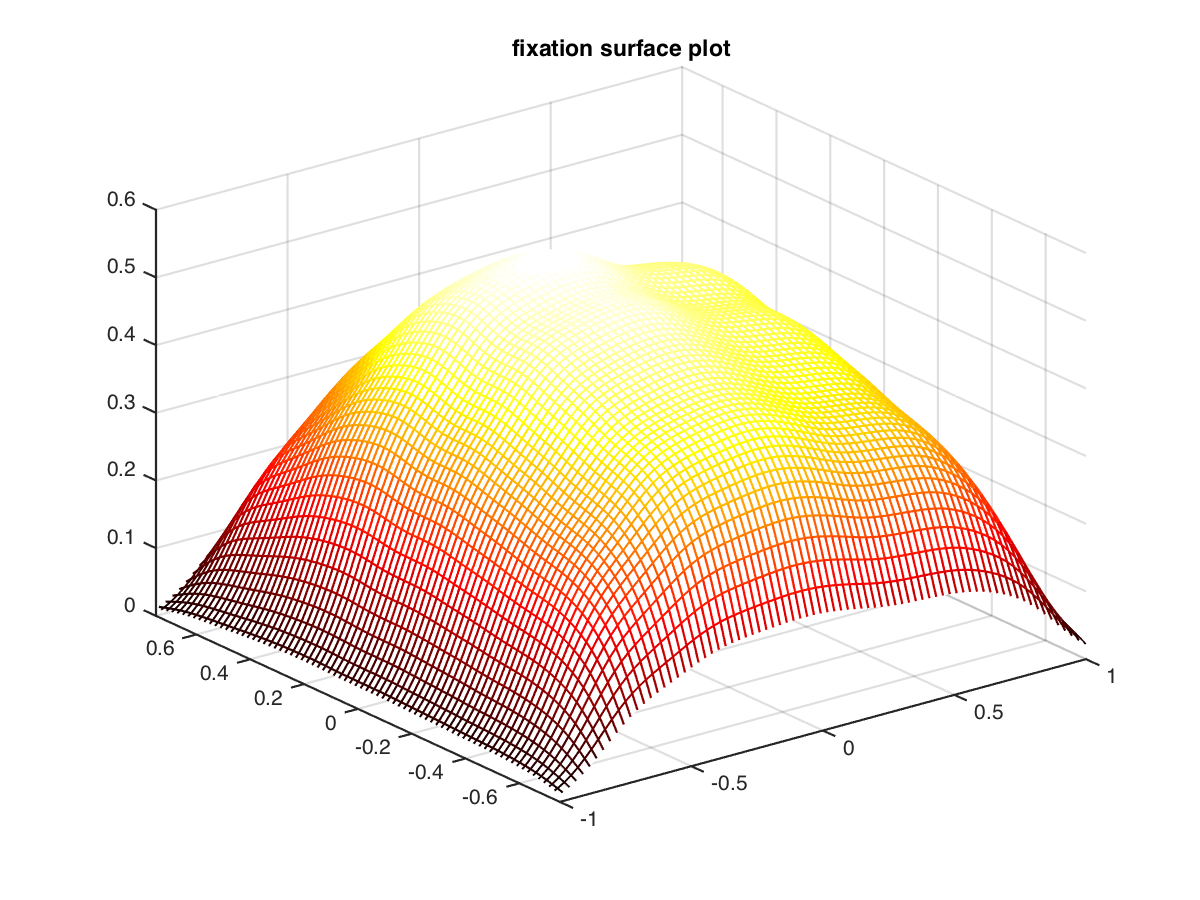
\includegraphics[width=7cm]{Figs/Clarke2009_3D.png}}
\caption{Some guy called Clark's data}
\label{fig:Clarke2009}
\end{figure}

\subsection{Einhauser 2008}

\begin{figure}[H]
	\centering
	\subfigure{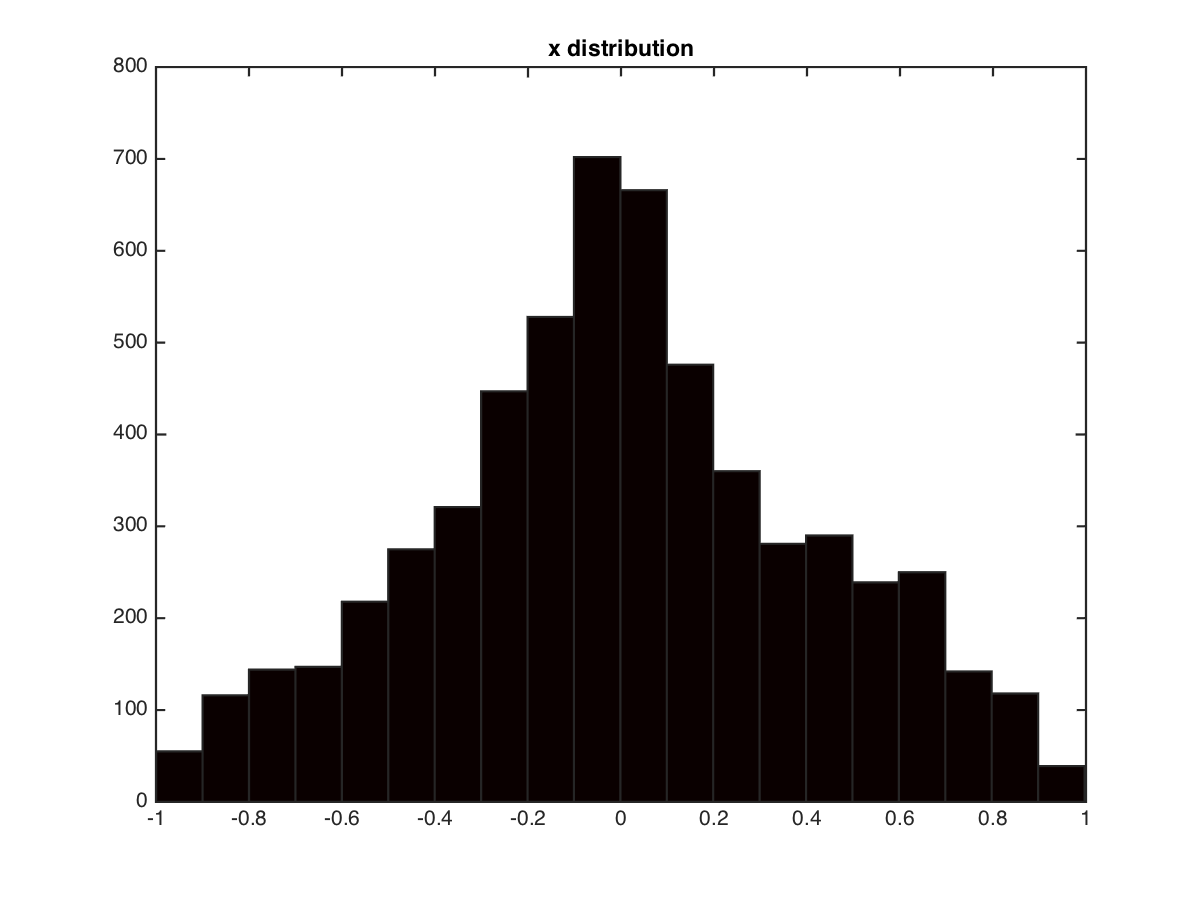
\includegraphics[width=7cm]{Figs/Einhauser2008_xdist.png}}
	\subfigure{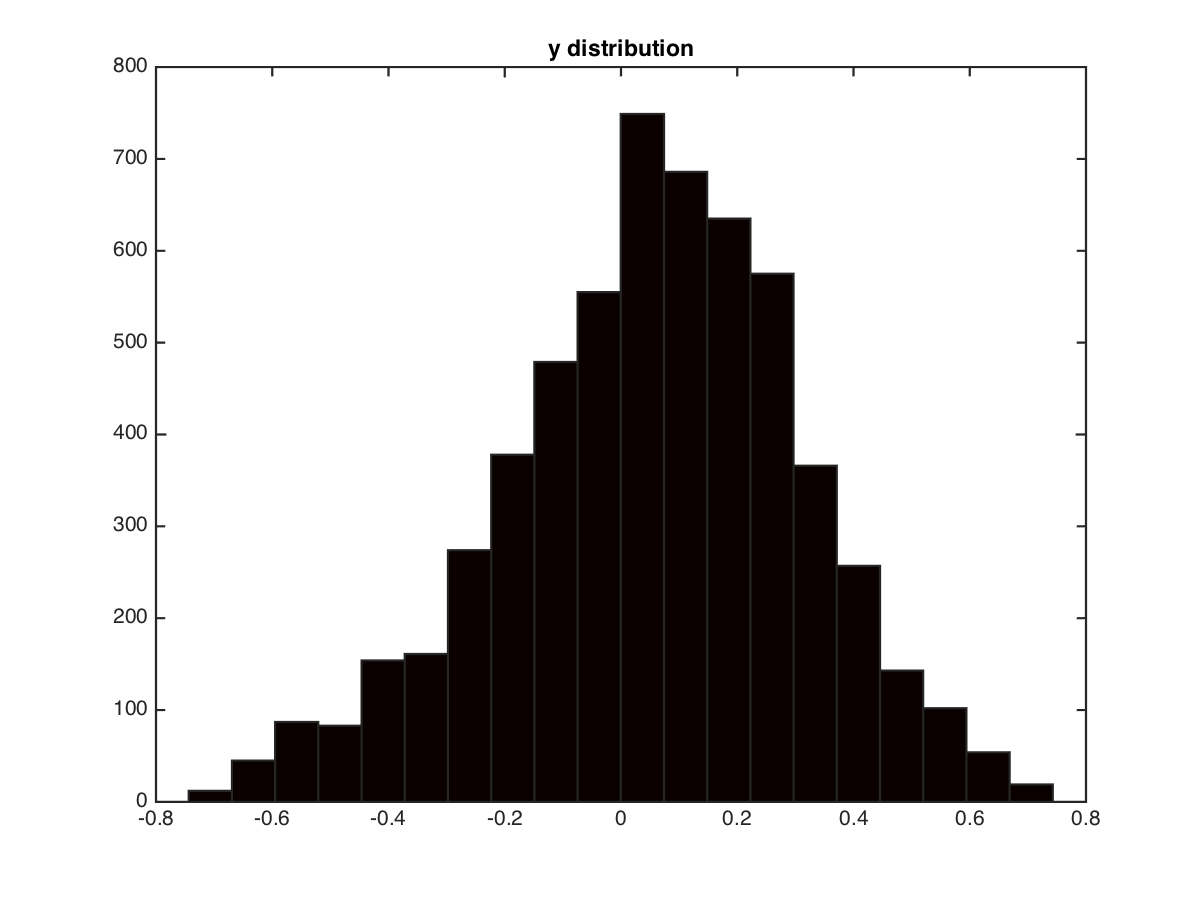
\includegraphics[width=7cm]{Figs/Einhauser2008_ydist.png}}
	\subfigure{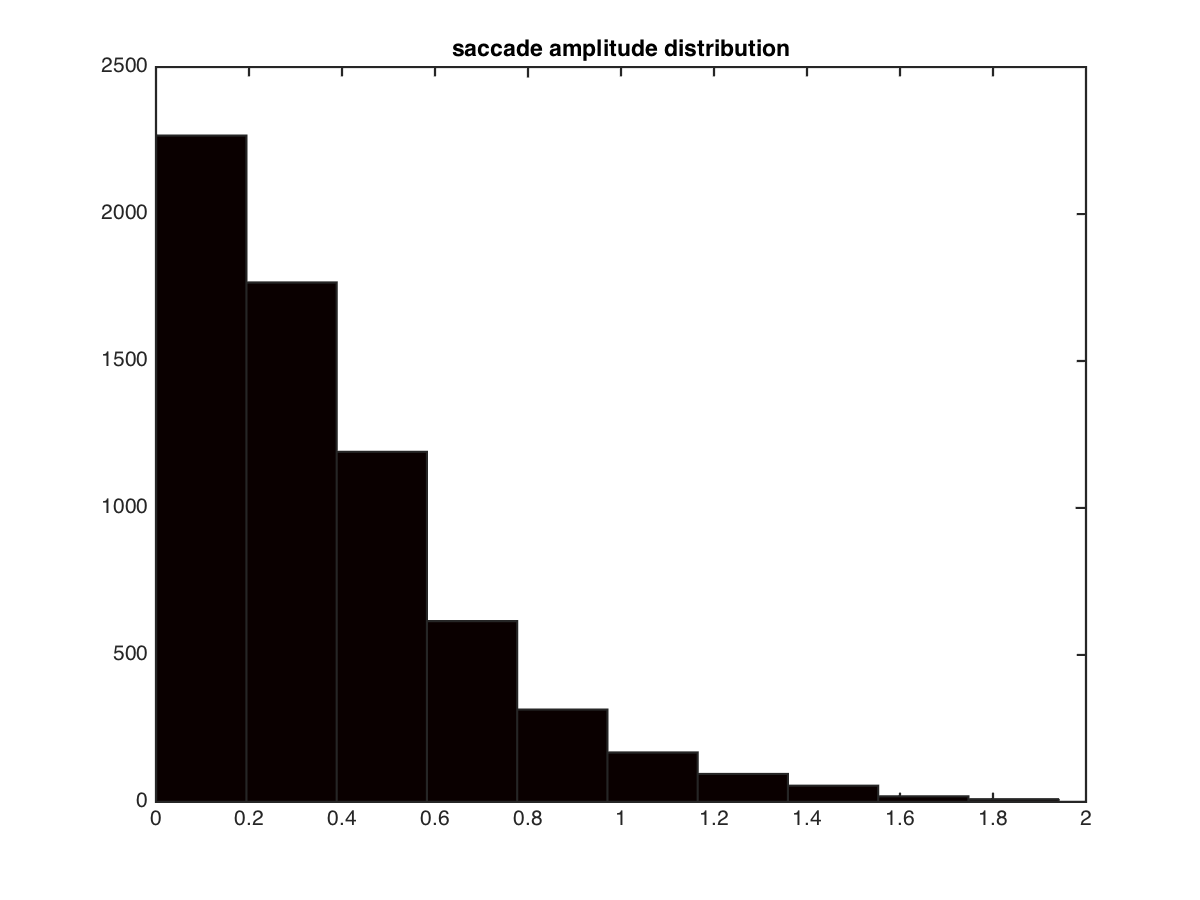
\includegraphics[width=7cm]{Figs/Einhauser2008_sacampdist.png}}
	\subfigure{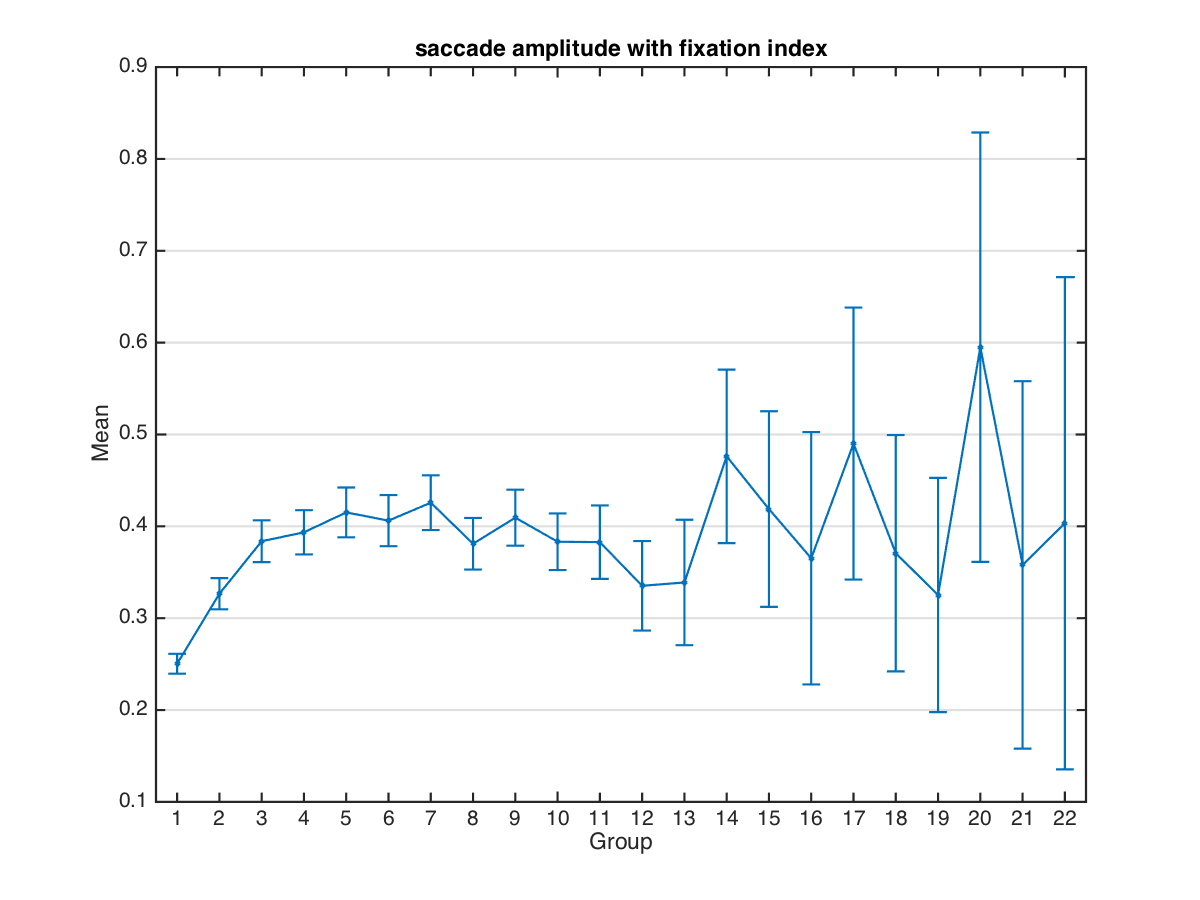
\includegraphics[width=7cm]{Figs/Einhauser2008_sacampindex.png}}
	\subfigure{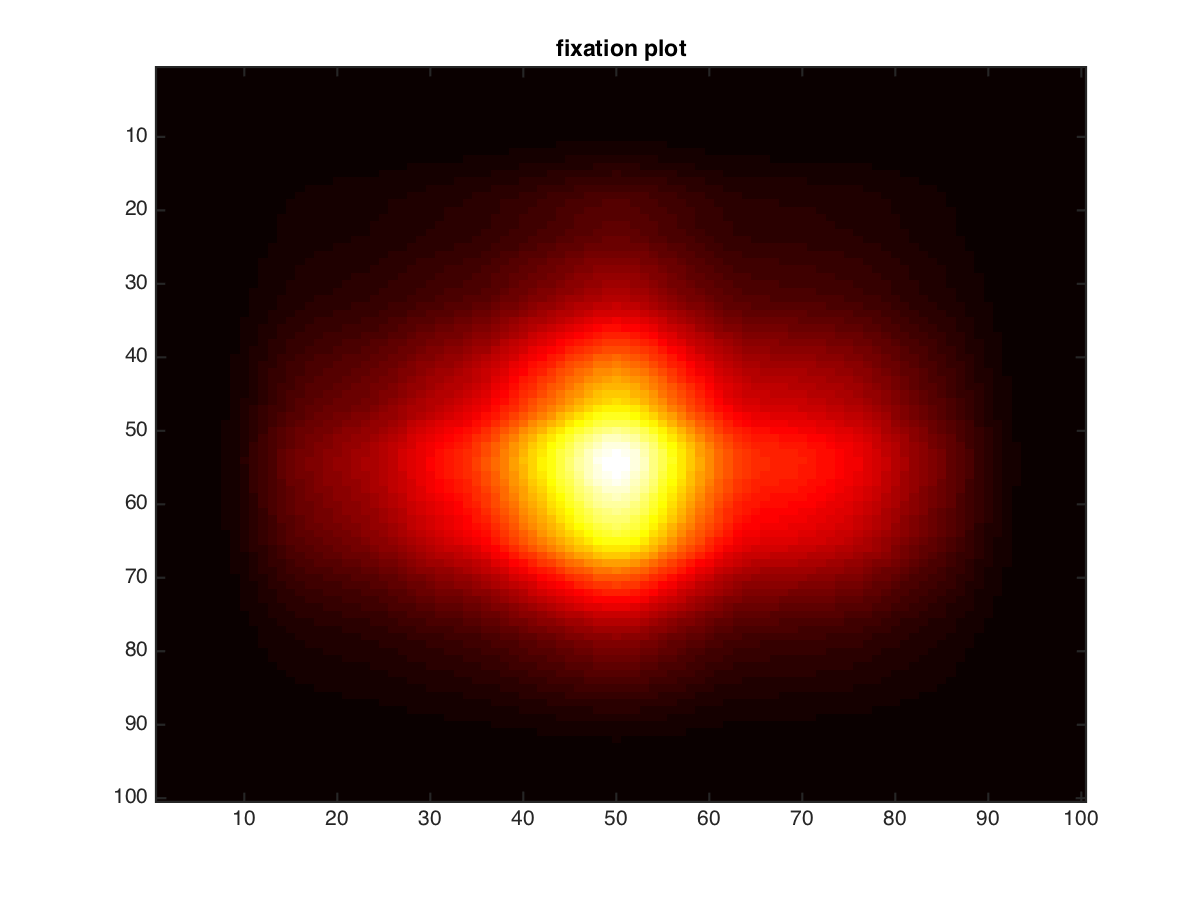
\includegraphics[width=7cm]{Figs/Einhauser2008_heat.png}}
	\subfigure{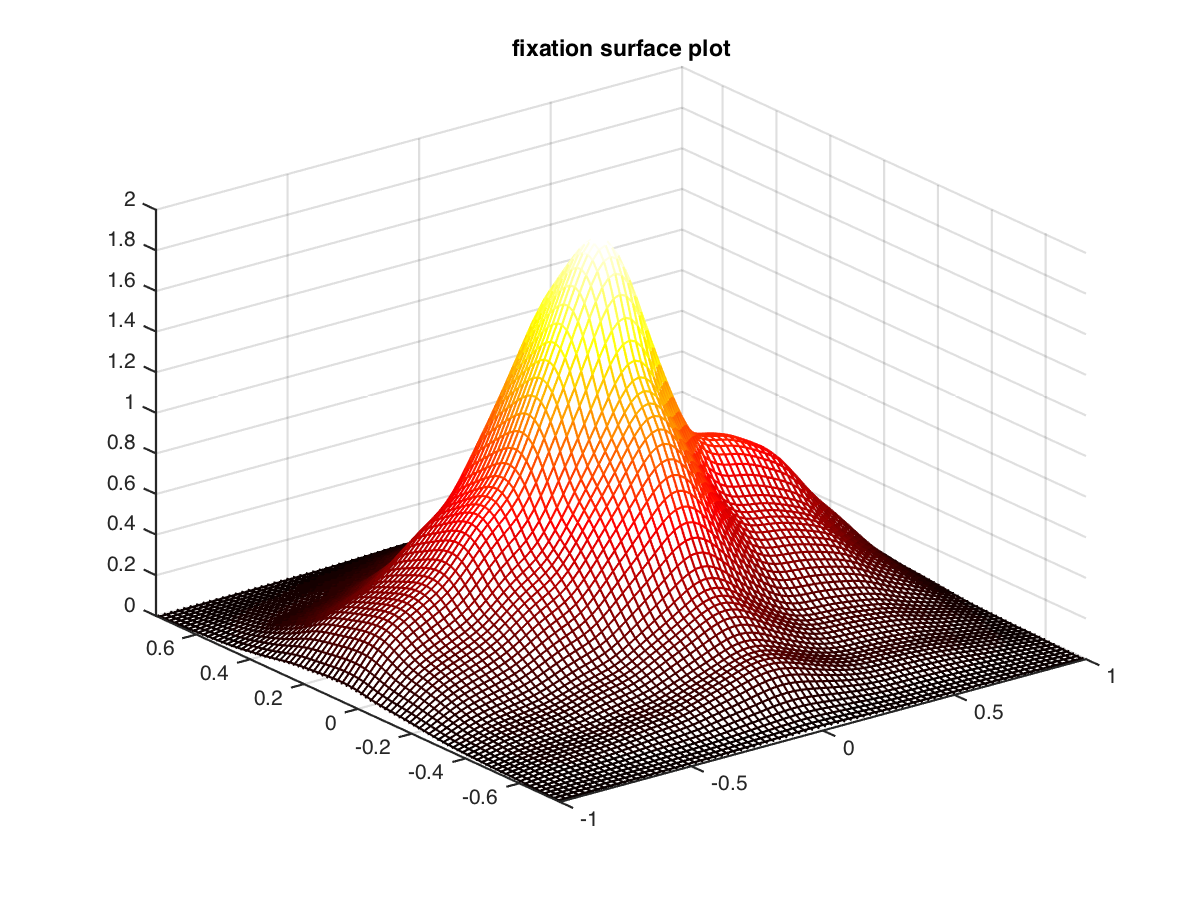
\includegraphics[width=7cm]{Figs/Einhauser2008_3D.png}}
\caption{Einhauser 2008 data}
\label{fig:Einhauser2008}
\end{figure}

\subsection{Tatler 2007 Search}

\begin{figure}[H]
	\centering
	\subfigure{\includegraphics[width=7cm]{Figs/Tatler2007Search_xdist.png}}
	\subfigure{\includegraphics[width=7cm]{Figs/Tatler2007Search_ydist.png}}
	\subfigure{\includegraphics[width=7cm]{Figs/Tatler2007Search_sacampdist.png}}
	\subfigure{\includegraphics[width=7cm]{Figs/Tatler2007Search_sacampindex.png}}
	\subfigure{\includegraphics[width=7cm]{Figs/Tatler2007Search_heat.png}}
	\subfigure{\includegraphics[width=7cm]{Figs/Tatler2007Search_3D.png}}
\caption{Tatler 2007 search data}
\label{fig:Tatler2007Search}
\end{figure}

\subsection{Tatler 2007 Free viewing}

\begin{figure}[H]
	\centering
	\subfigure{\includegraphics[width=7cm]{Figs/Tatler2007Freeview_xdist.png}}
	\subfigure{\includegraphics[width=7cm]{Figs/Tatler2007Freeview_ydist.png}}
	\subfigure{\includegraphics[width=7cm]{Figs/Tatler2007Freeview_sacampdist.png}}
	\subfigure{\includegraphics[width=7cm]{Figs/Tatler2007Freeview_sacampindex.png}}
	\subfigure{\includegraphics[width=7cm]{Figs/Tatler2007Freeview_heat.png}}
	\subfigure{\includegraphics[width=7cm]{Figs/Tatler2007Freeview_3D.png}}
\caption{Tatler 2007 Freeview data}
\label{fig:Tatler2007Freeview}
\end{figure}


\subsection{Tatler 2005}

\begin{figure}[H]
	\centering
	\subfigure{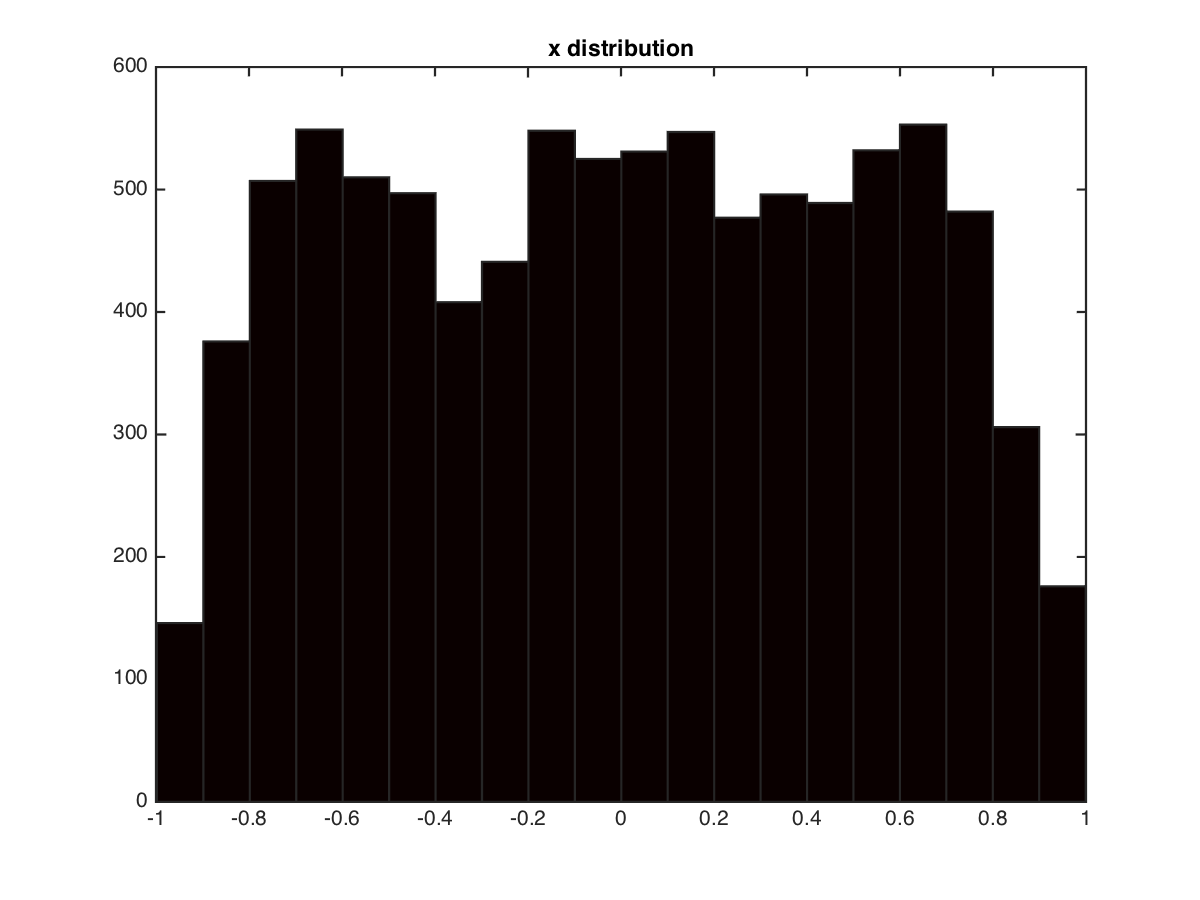
\includegraphics[width=7cm]{Figs/Tatler2005_xdist.png}}
	\subfigure{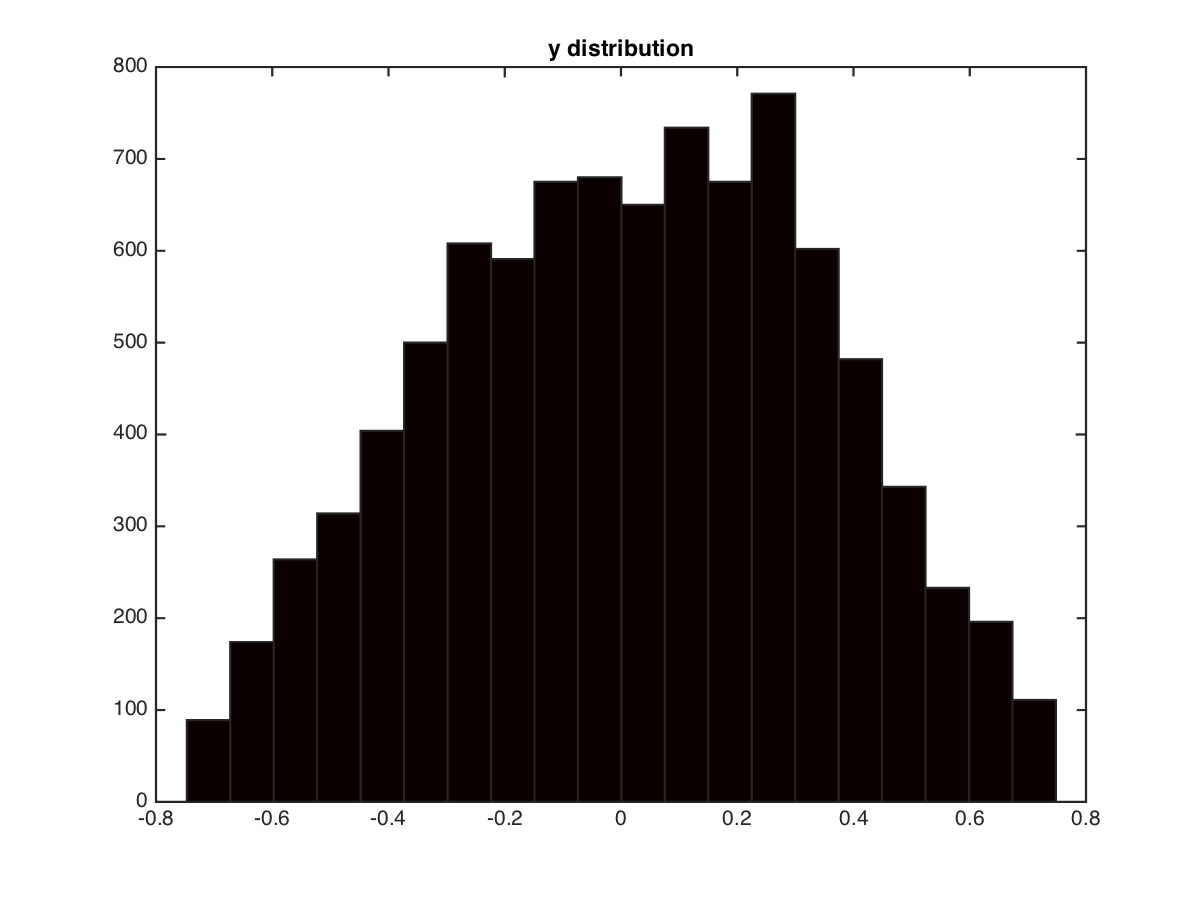
\includegraphics[width=7cm]{Figs/Tatler2005_ydist.png}}
	\subfigure{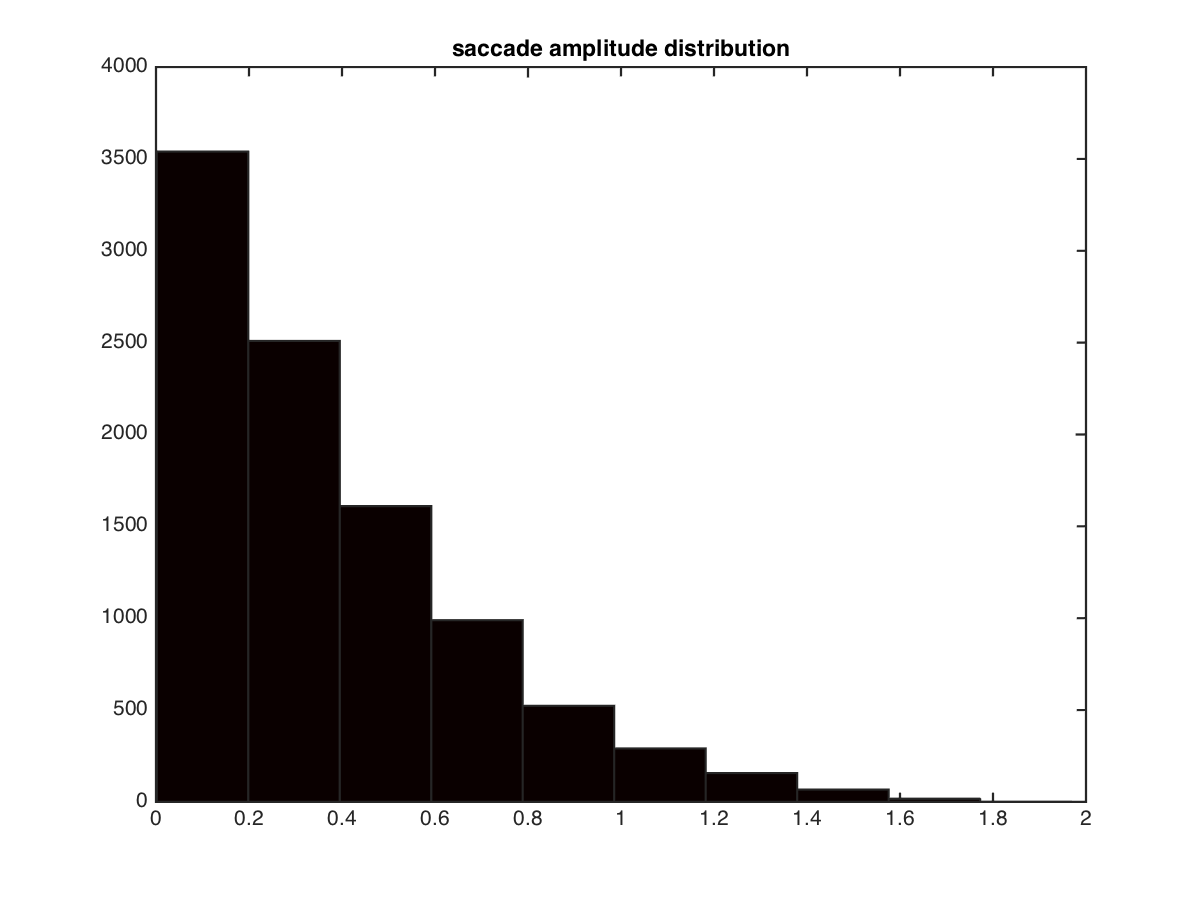
\includegraphics[width=7cm]{Figs/Tatler2005_sacampdist.png}}
	\subfigure{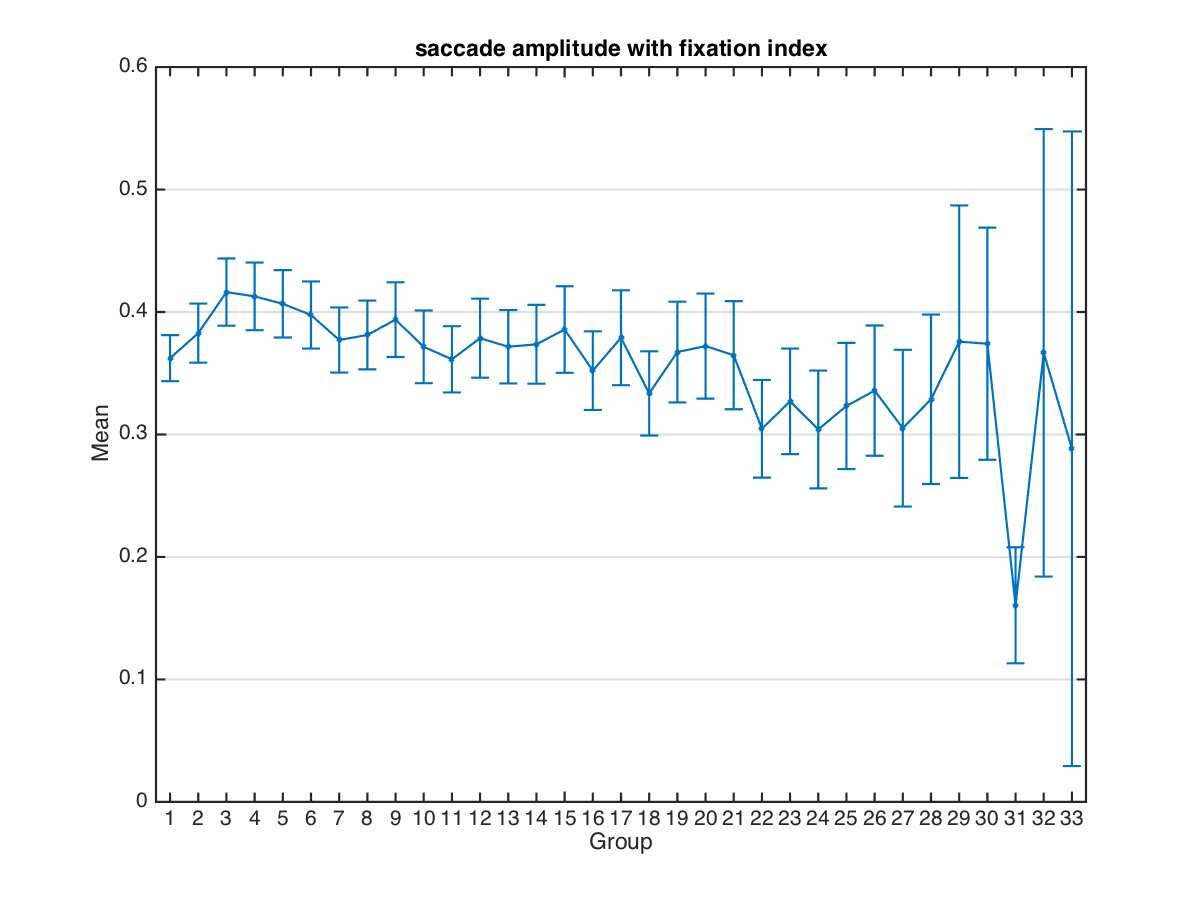
\includegraphics[width=7cm]{Figs/Tatler2005_sacampindex.png}}
	\subfigure{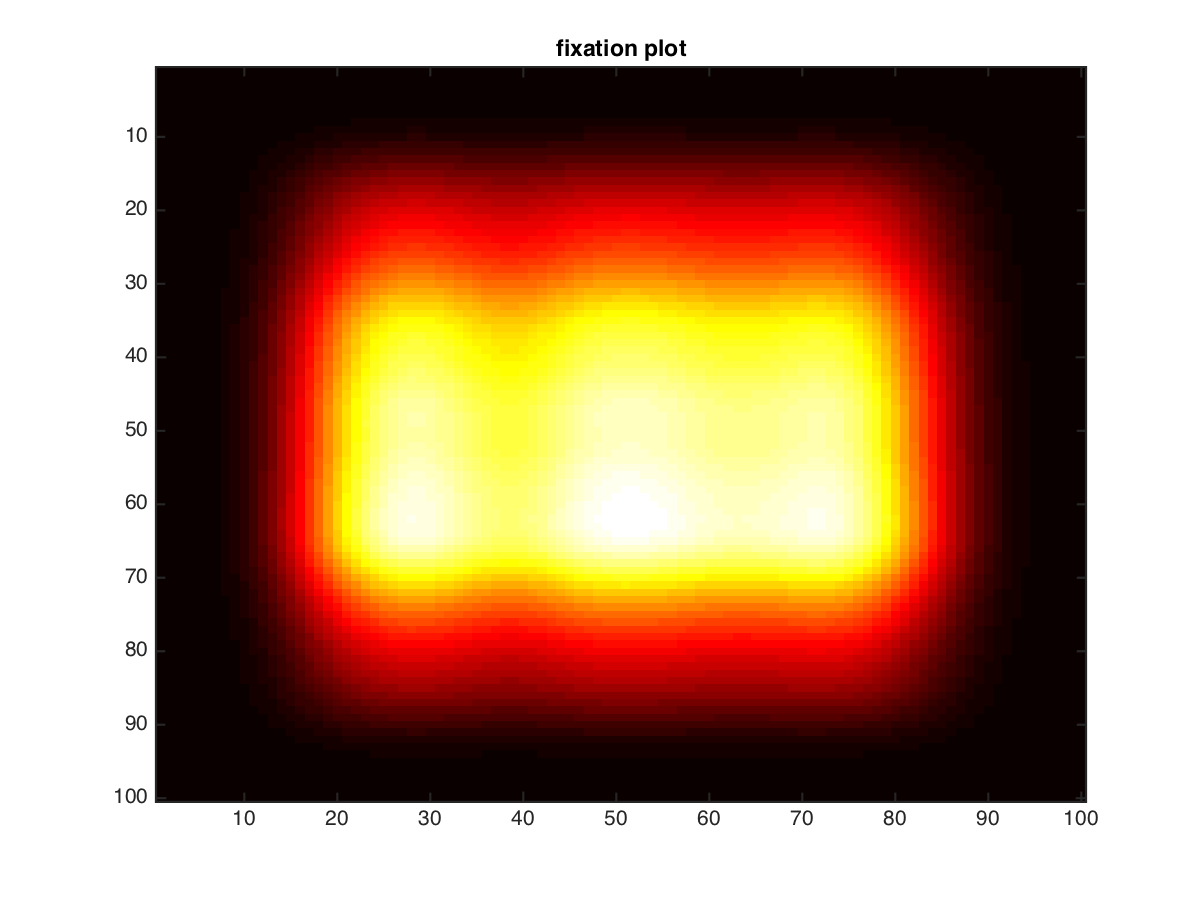
\includegraphics[width=7cm]{Figs/Tatler2005_heat.png}}
	\subfigure{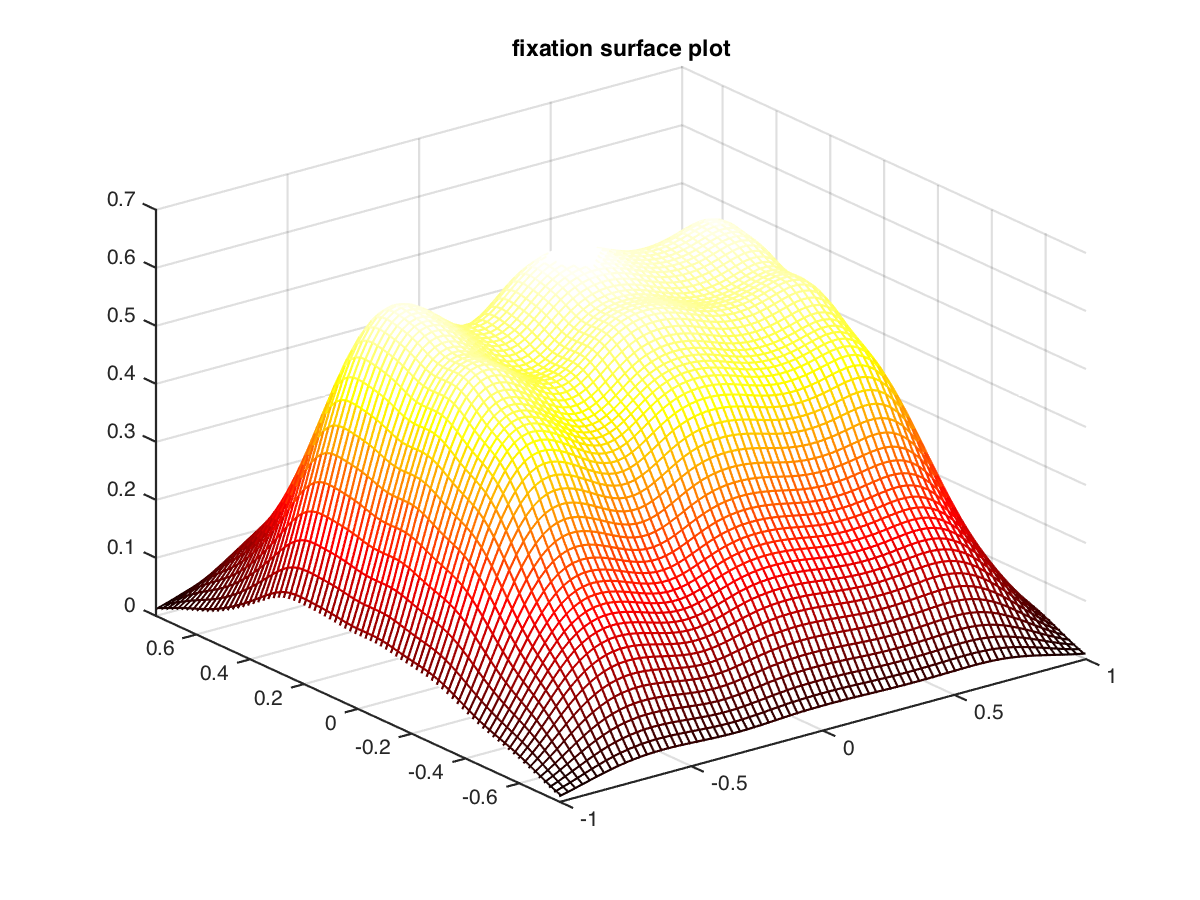
\includegraphics[width=7cm]{Figs/Tatler2005_3D.png}}
\caption{Tatler 2005 data}
\label{fig:Tatler2005}
\end{figure}

\subsection{Judd 2009}

\begin{figure}[H]
	\centering
	\subfigure{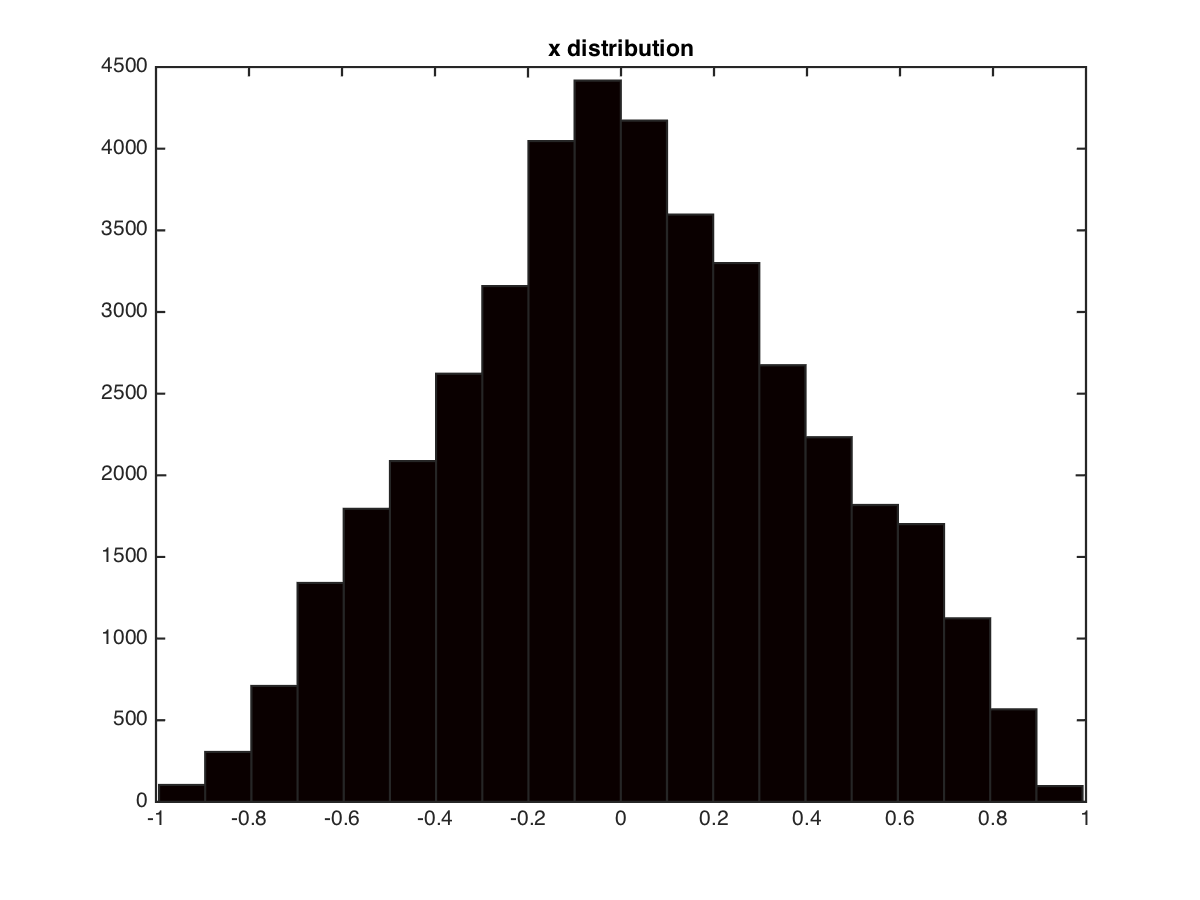
\includegraphics[width=7cm]{Figs/Judd2009_xdist.png}}
	\subfigure{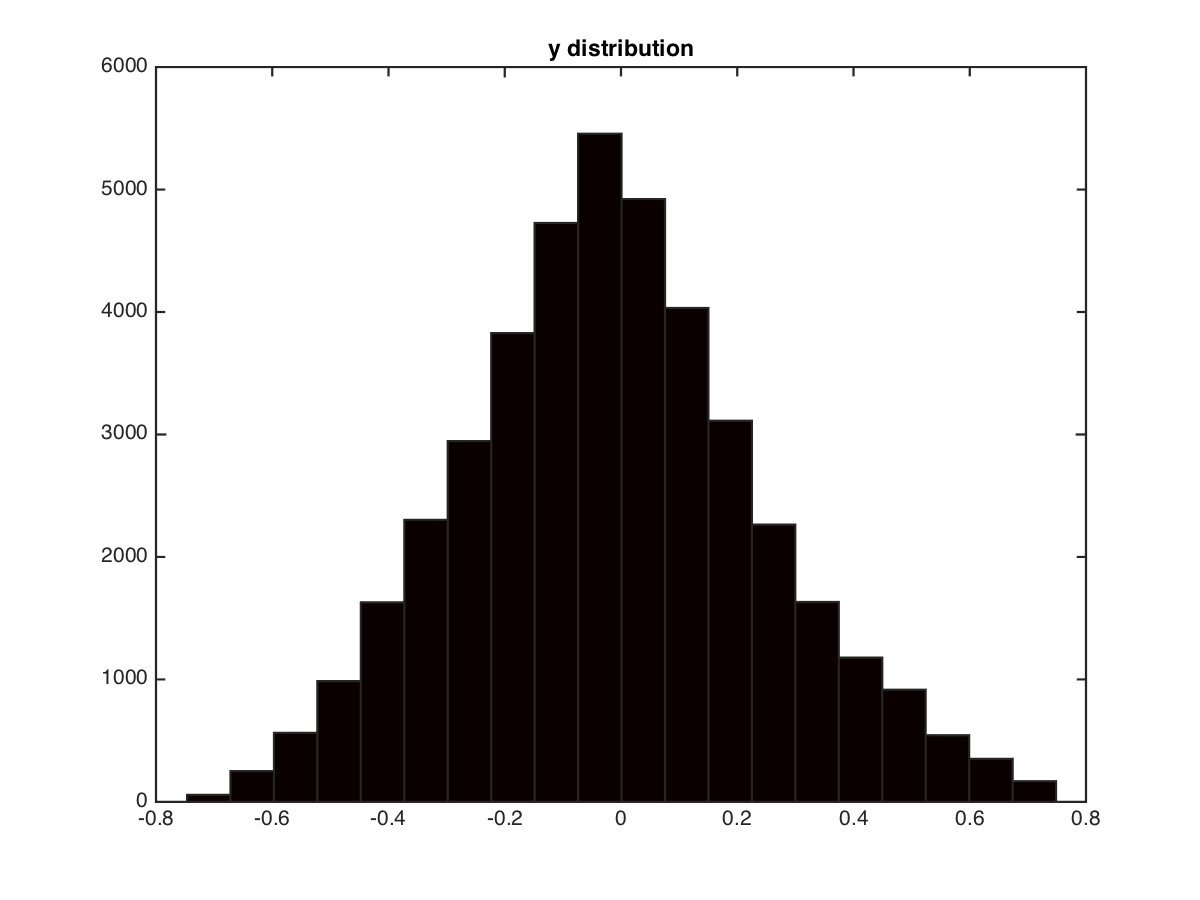
\includegraphics[width=7cm]{Figs/Judd2009_ydist.png}}
	\subfigure{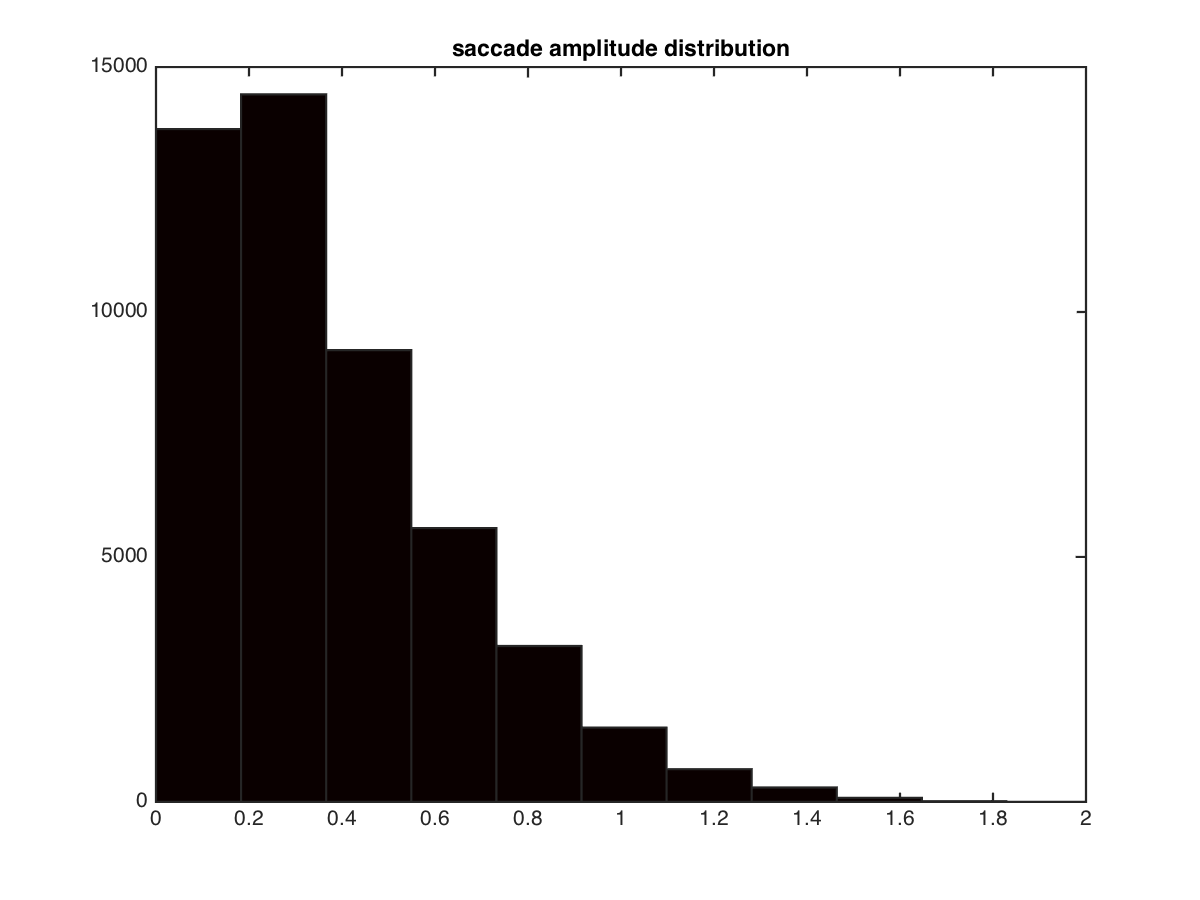
\includegraphics[width=7cm]{Figs/Judd2009_sacampdist.png}}
	\subfigure{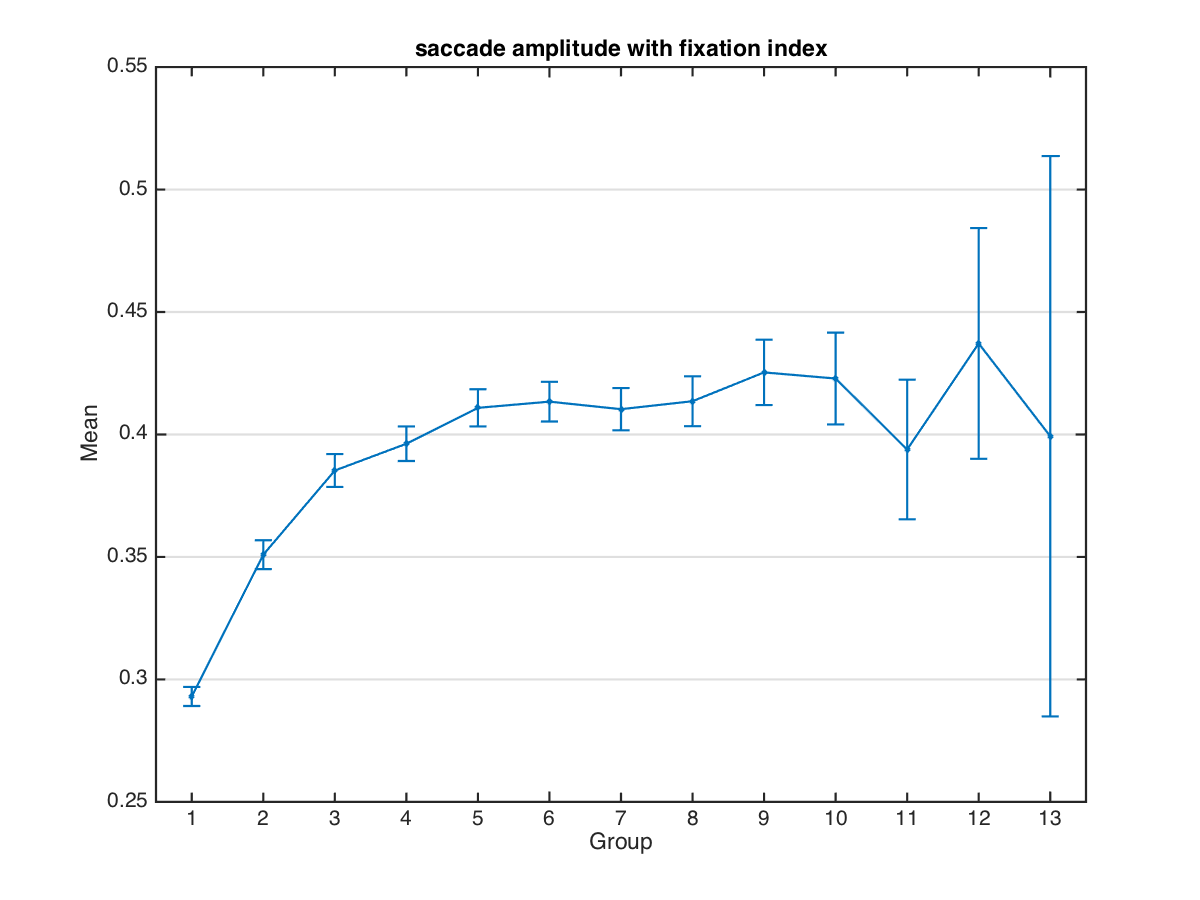
\includegraphics[width=7cm]{Figs/Judd2009_sacampindex.png}}
	\subfigure{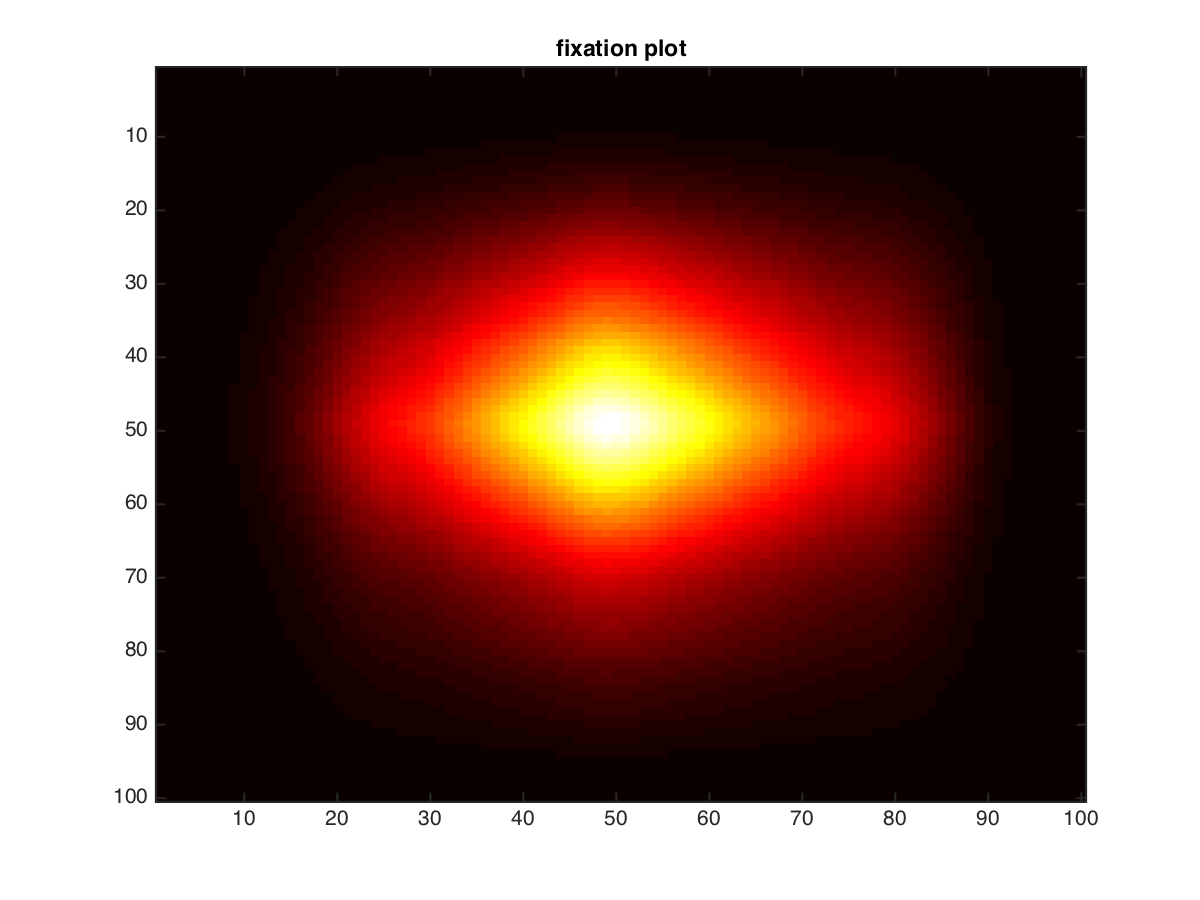
\includegraphics[width=7cm]{Figs/Judd2009_heat.png}}
	\subfigure{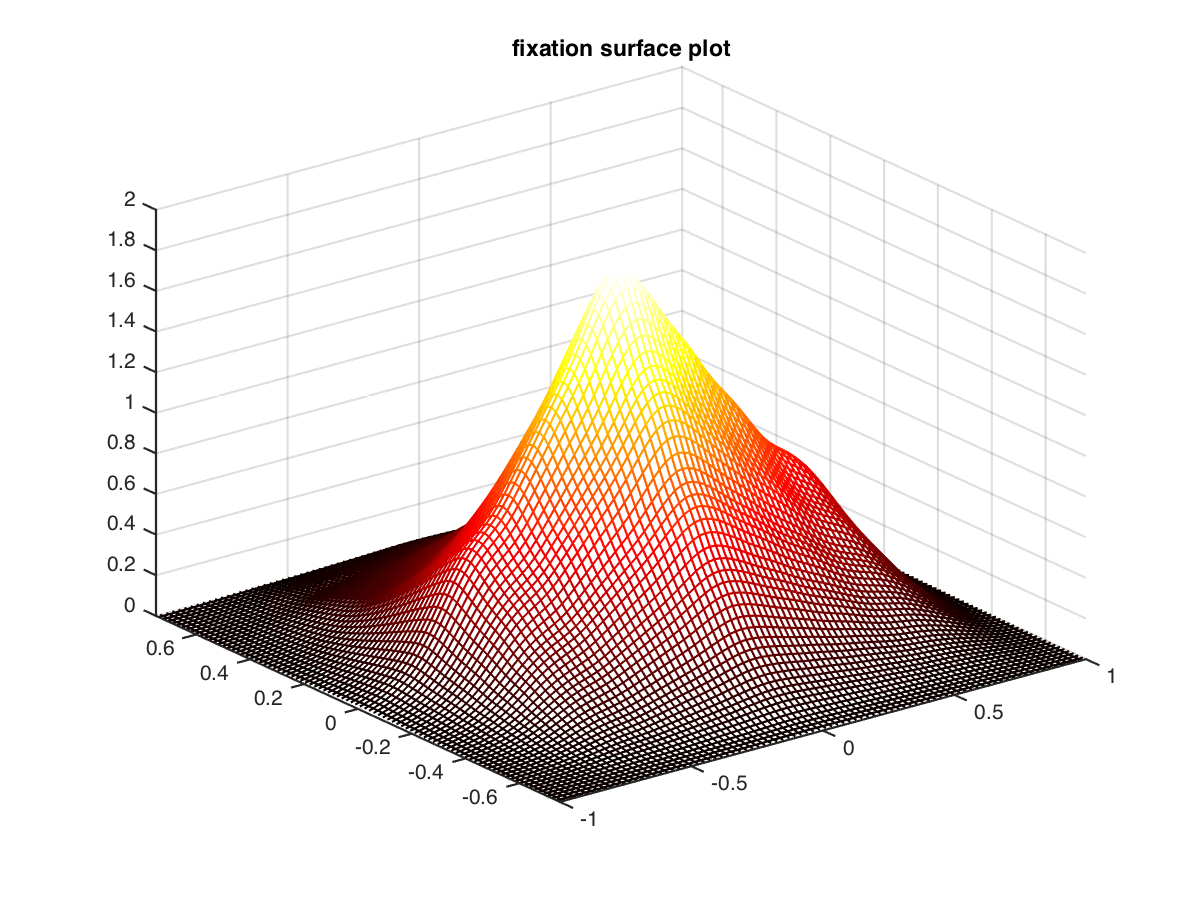
\includegraphics[width=7cm]{Figs/Judd2009_3D.png}}
\caption{Judd 2009 data}
\label{fig:Judd2009}
\end{figure}

\subsection{Yun 2013 SUN}

\begin{figure}[H]
	\centering
	\subfigure{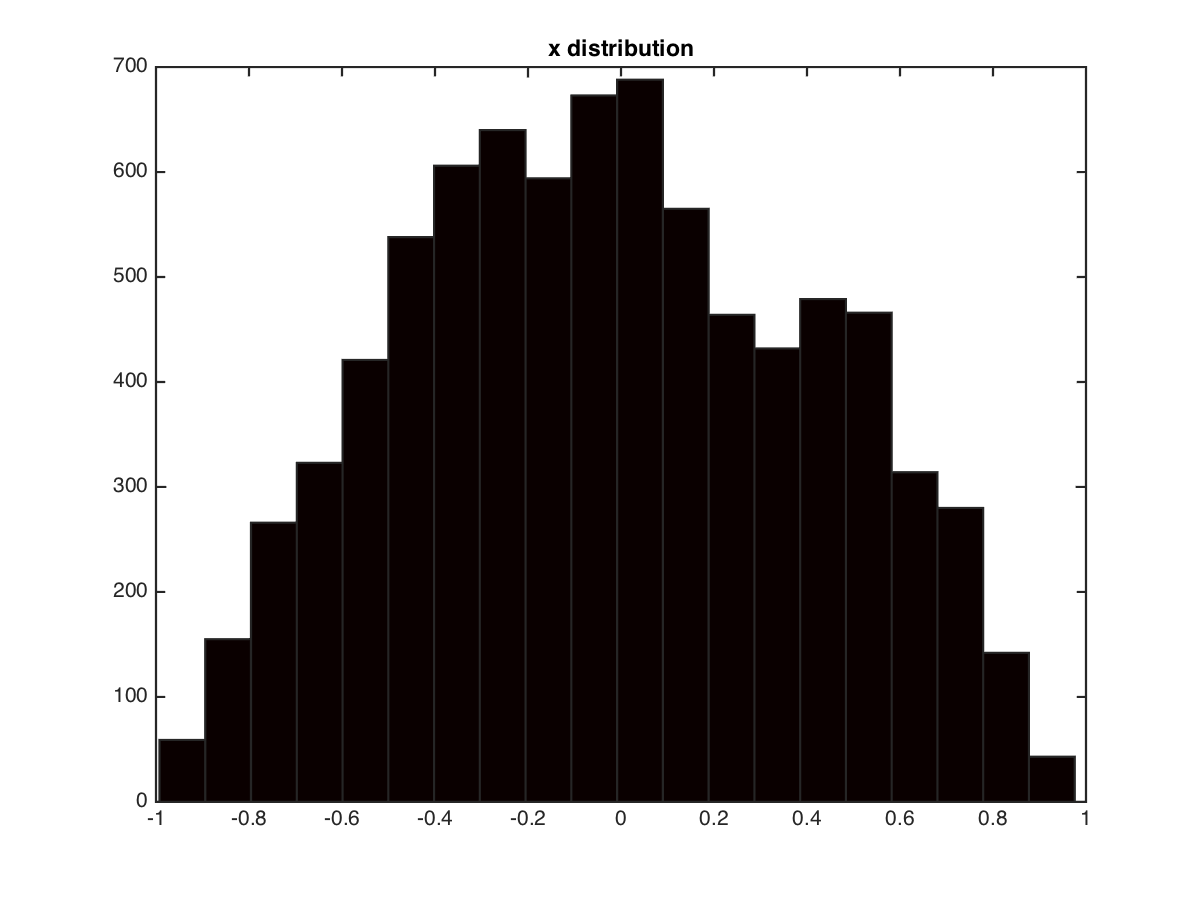
\includegraphics[width=7cm]{Figs/Yun2013SUN_xdist.png}}
	\subfigure{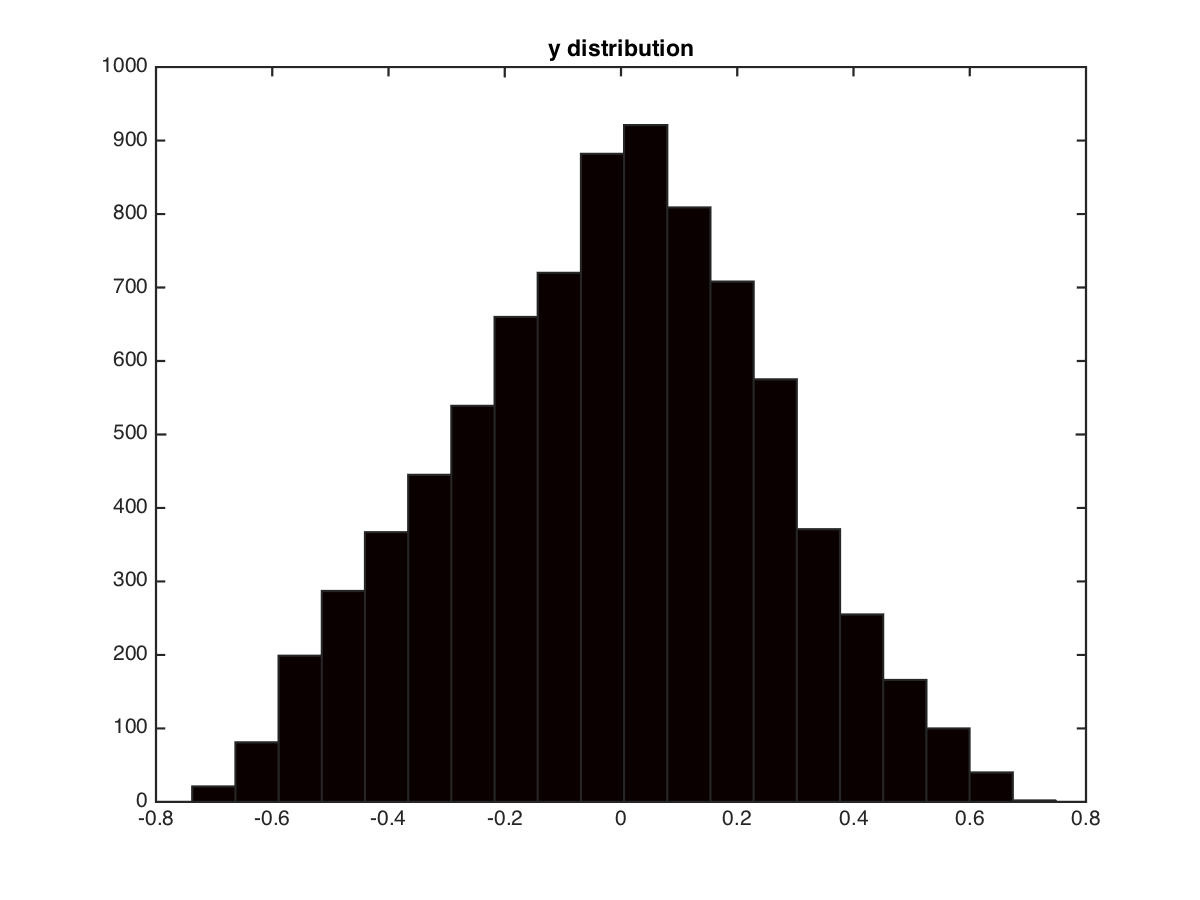
\includegraphics[width=7cm]{Figs/Yun2013SUN_ydist.png}}
	\subfigure{\includegraphics[width=7cm]{Figs/Yun2013SUN_sacampdist.png}}
	\subfigure{\includegraphics[width=7cm]{Figs/Yun2013SUN_sacampindex.png}}
	\subfigure{\includegraphics[width=7cm]{Figs/Yun2013SUN_heat.png}}
	\subfigure{\includegraphics[width=7cm]{Figs/Yun2013SUN_3D.png}}
\caption{Yun 2013 SUN data}
\label{fig:Yun2013SUN}
\end{figure}


\subsection{Yun 2013 PASCAL}

\begin{figure}[H]
	\centering
	\subfigure{\includegraphics[width=7cm]{Figs/Yun2013PASCAL_xdist.png}}
	\subfigure{\includegraphics[width=7cm]{Figs/Yun2013PASCAL_ydist.png}}
	\subfigure{\includegraphics[width=7cm]{Figs/Yun2013PASCAL_sacampdist.png}}
	\subfigure{\includegraphics[width=7cm]{Figs/Yun2013PASCAL_sacampindex.png}}
	\subfigure{\includegraphics[width=7cm]{Figs/Yun2013PASCAL_heat.png}}
	\subfigure{\includegraphics[width=7cm]{Figs/Yun2013PASCAL_3D.png}}
\caption{Yun 2013 PASCAL data}
\label{fig:Yun2013PASCAL}
\end{figure}


\subsection{Greene 60 Sec Data}

\begin{figure}[H]
	\centering
	\subfigure{\includegraphics[width=7cm]{Figs/GreeneData_xdist.png}}
	\subfigure{\includegraphics[width=7cm]{Figs/GreeneData_ydist.png}}
	\subfigure{\includegraphics[width=7cm]{Figs/GreeneData_sacampdist.png}}
	\subfigure{\includegraphics[width=7cm]{Figs/GreeneData_sacampindex.png}}
	\subfigure{\includegraphics[width=7cm]{Figs/GreeneData_heat.png}}
	\subfigure{\includegraphics[width=7cm]{Figs/GreeneData_3D.png}}
\caption{Greene Data}
\label{fig:GreeneData}
\end{figure}



%\printbibliography
 
\end{document}